% !TeX spellcheck = nl_NL

\documentclass[12pt,a4paper,oneside]{book}
\usepackage{a4wide}
%\usepackage[top=3cm,bottom=4cm,outer=2cm,inner=3cm]{geometry}
\usepackage[dutch,english]{babel}       % Voor nederlandstalige hyphenatie (woordsplitsing)
\usepackage{amsmath}                    % Uitgebreide wiskundige mogelijkheden
\usepackage[binary-units=true]{siunitx} % si units
\usepackage{amssymb}                    % Voor speciale symbolen zoals de verzameling Z, R...
\usepackage{url}                        % Om url's te verwerken
\usepackage{graphicx}                   % Om figuren te kunnen verwerken
\usepackage[small,bf,hang]{caption2}    % Om de captions wat te verbeteren
\usepackage{xspace}                     % Magische spaties na een commando
\usepackage[latin1]{inputenc}           % Om niet ascii karakters rechtstreeks te kunnen typen
\usepackage{float}                      % Om nieuwe float environments aan te maken. Ook optie H!
\usepackage{flafter}                    % Opdat floats niet zouden voorsteken
\usepackage{listings}                   % Voor het weergeven van letterlijke text en codelistings
\usepackage{marvosym}                   % Om het euro symbool te krijgen
\usepackage{textcomp}                   % Voor onder andere graden celsius
\usepackage{fancyhdr}                   % Voor fancy headers en footers.
\usepackage{graphics}					% Om figuren te verwerken.
\usepackage[nottoc]{tocbibind} 			% Bibliografie in ToC; zie tocbibind.dvi
%\usepackage{pstricks}
\usepackage{longtable}
\usepackage{pdfpages}  					% pdf pagina's importeren
\usepackage{url} 						% allows urls in bibtex?
\usepackage{subfigure}					% gebruikt subfigure package
\usepackage{mathtools}					% package voor matrix alignment
\usepackage{tabularx}					% package voor tabelsize

\newcommand{\npar}{\par \vspace{2.3ex plus 0.3ex minus 0.3ex} \noindent}	% Om witruimte te krijgen tussen paragrafen
\graphicspath{{./Figuren/}}               % De plaats waar latex zijn figuren gaat halen.
\usepackage[bf]{caption2}	% Mooiere captions
\usepackage[a4paper,plainpages=false]{hyperref}    % Om hyperlinks te hebben in het pdfdocument.
\newcommand{\command}[1]{\lstinline[basicstyle=\tt]{#1}\xspace} %Voor commando's
\hyphenation{om-ge-vings-map-pin-met-een-au-to-no-me-quad-cop-ter}


\renewcommand{\chaptermark}[1]{\markright{\MakeUppercase{#1}}}
\renewcommand{\sectionmark}[1]{\markright{\thesection~#1}}

\newcommand{\headerfmt}[1]{\textsl{\textsf{#1}}}
\newcommand{\headerfmtpage}[1]{\textsf{#1}}

\fancyhf{}
\fancyhead[LE,RO]{\headerfmtpage{\thepage}}
\fancyhead[LO]{\headerfmt{\rightmark}}
\fancyhead[RE]{\headerfmt{\leftmark}}
\renewcommand{\headrulewidth}{0.5pt}
\renewcommand{\footrulewidth}{0pt}

\fancypagestyle{plain}{ % eerste bladzijde van een hoofdstuk
  \fancyhf{}
  \fancyhead[LE,RO]{\headerfmtpage{\thepage}}
  \fancyhead[LO]{\headerfmt{\rightmark}}
  \fancyhead[RE]{\headerfmt{\leftmark}}
  \renewcommand{\headrulewidth}{0.5pt}
  \renewcommand{\footrulewidth}{0pt}
}

\renewcommand{\lstlistoflistings}{\begingroup
   \tocfile{\lstlistlistingname}{lol}
\endgroup}


\hypersetup{
    pdfauthor = {Karel Serruys},
    pdftitle = {Omgevingsmapping met autonome quadcopter},
    pdfsubject = {Masterproef ingediend tot het behalen van de academische graad van Master of Science in de ingenieurswetenschappen: elektrotechniek}
}

\begin{document}
\nocite{*}
\selectlanguage{dutch}

\frontmatter

% geen paginanummering tot we aan de inhoudsopgave komen
\pagestyle{empty}

%kaft titel pagina
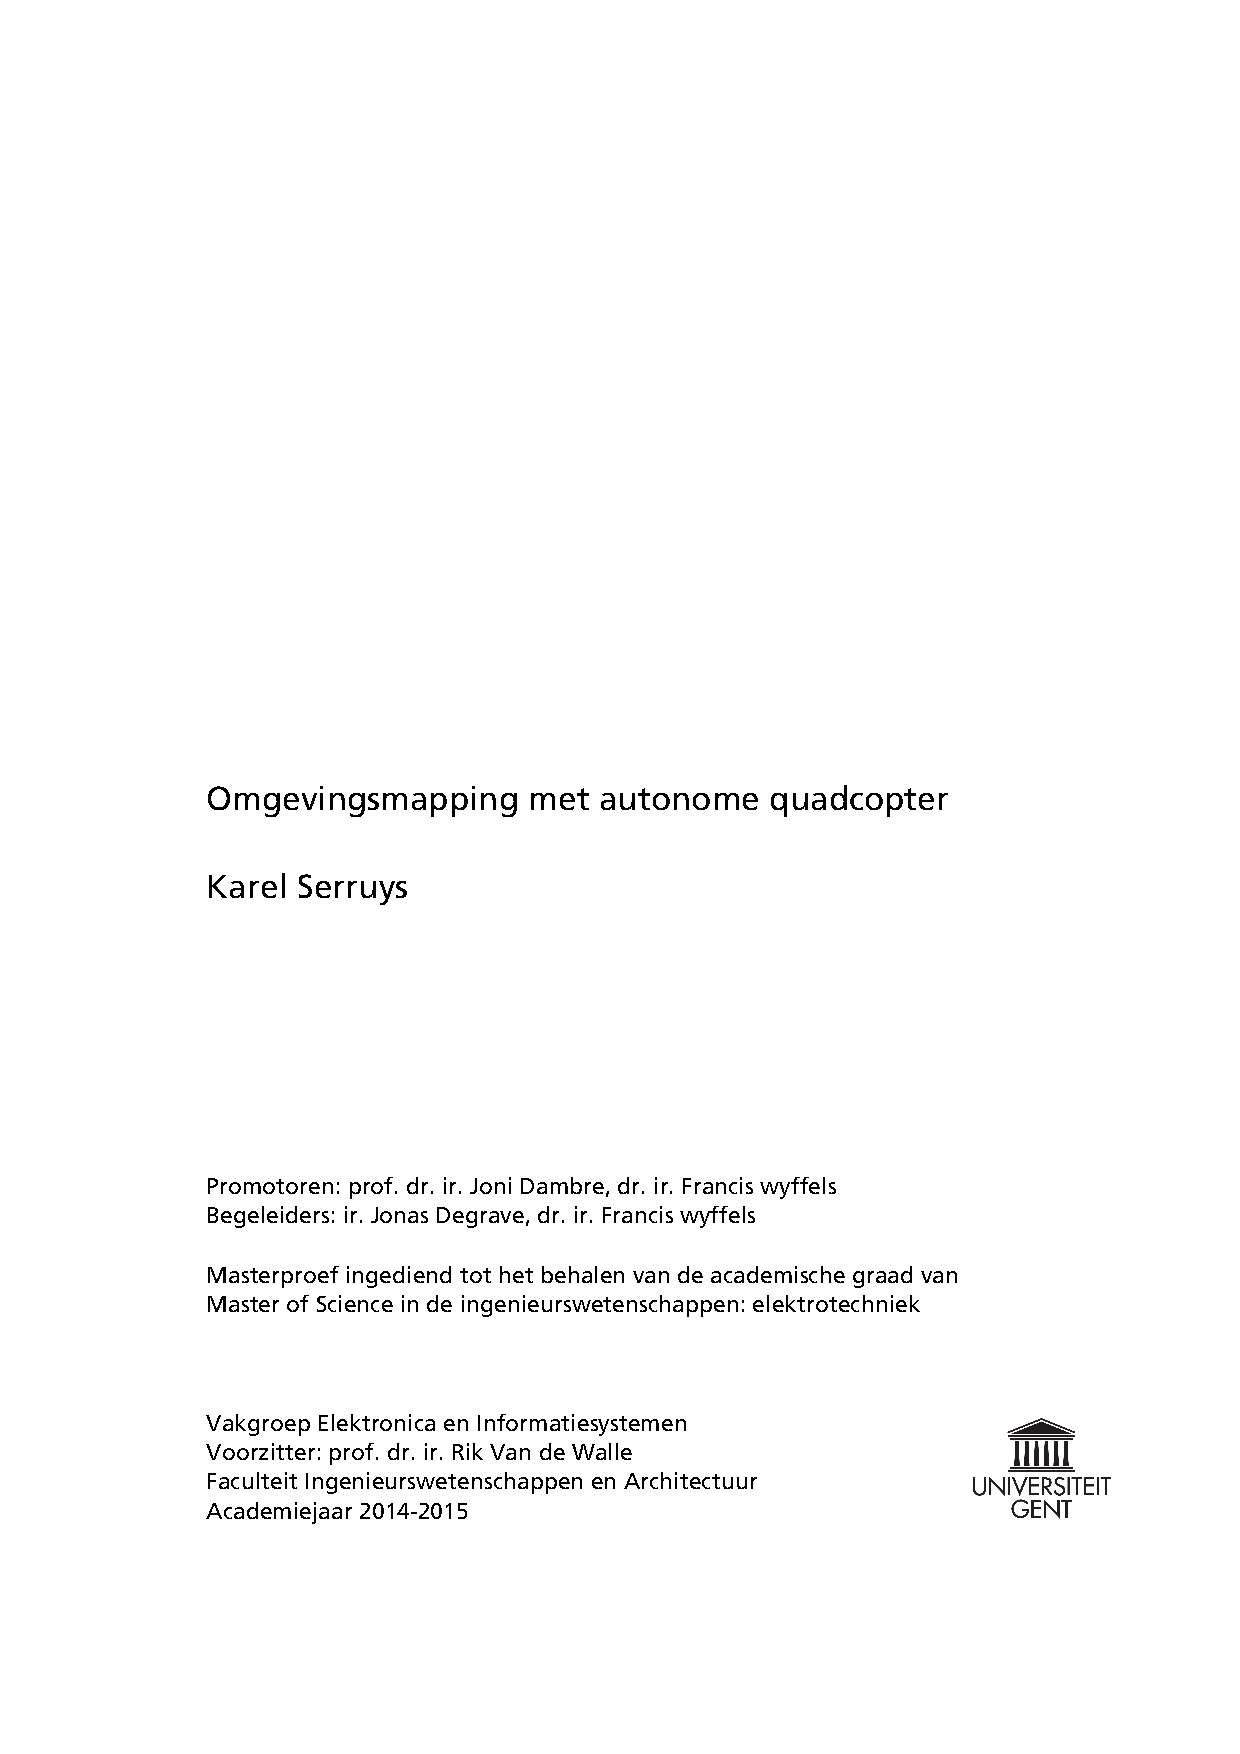
\includepdf[pages={1}]{titel.pdf}

% lege pagina (!!)
\newpage
\vfil\null
\newpage


% titelblad (!!)
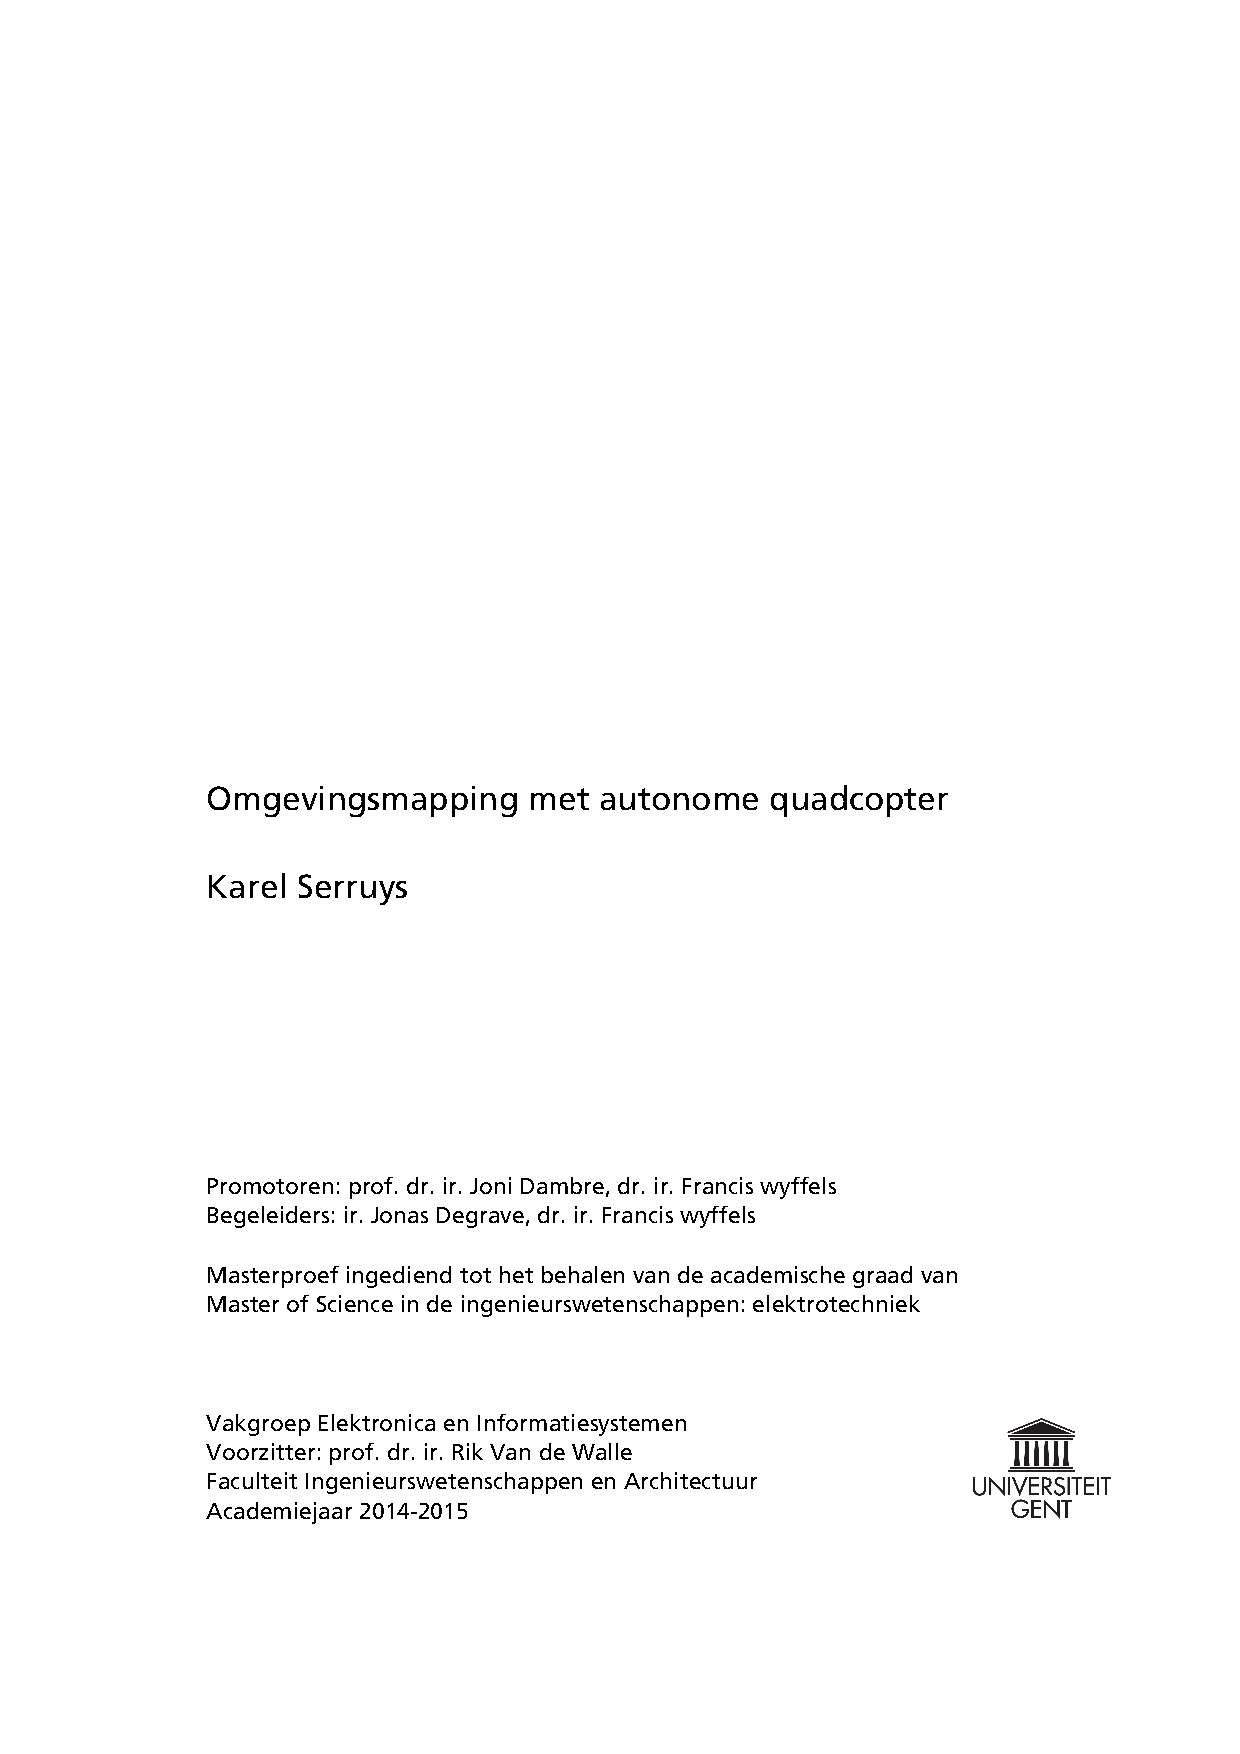
\includepdf[pages={1}]{titel.pdf}


% voorwoord met dankwoord en toelating tot bruikleen (ondertekend)
\pagestyle{empty}
\renewcommand{\baselinestretch}{1.3}
% !TeX spellcheck = nl_NL
\newpage
\thispagestyle{empty}
\npar {\Huge \textbf{Voorwoord}}\\
\\
\\
\textit{Ik heb deze thesis geschreven tot het behalen van het diploma burgerlijk ingenieur in de elektrotechniek. Bij het schrijven van dit werk ben ik veel problemen tegengekomen, het ging vaak moeilijk. Maar hoe moeilijker het probleem was, hoe meer voldoening ik eruit haalde eens het opgelost was. Uiteraard stond ik er niet alleen voor. Ik wil graag de mensen bedanken die mij geholpen hebben om deze thesis tot een goed einde te brengen.\\
\\	
Eerst en vooral wil ik mijn begeleider ir. Jonas Degrave bedanken, aan wie ik altijd advies kon vragen. Graag wil ik ook mijn promotoren prof. dr. ir. Joni Dambre en dr. ir. {Francis} {wyffels} bedanken om mij de kans te geven een thesis te doen over robotica in Reservoir Lab.\\
\\
Ik wil graag ook mijn vrienden bedanken. Om te beginnen bedank ik mijn medestudenten Joachim Ally, Pieter Heemeryck en Tom Thevelein van ons eigen opgerichte `Team Elektro'. Samen hebben we vijf jaar lang onze kennis gedeeld en elkaar door iedere examenperiode heen geholpen. Ook wil ik Mathieu Verfaillie en Gillis Sanctobin bedanken voor de ontspannende momenten tussen het schrijven door.\\
\\
Ten slotte wil ik nog mijn familie bedanken. Eerst en vooral ben ik mijn ouders Wim en Lut en mijn zussen Lise en Nele heel dankbaar omdat ze mij altijd geholpen hebben waar mogelijk en ze mij altijd zijn blijven aanmoedigen. Om af te sluiten wil ik nog met heel mijn hart mijn vriendin Stefanie Ghettem bedanken omdat ik ook altijd bij haar terecht kon.}\\
\\
\begin{flushright}
	Karel Serruys\\
	Gent, juni 2015
\end{flushright}

\newpage
\thispagestyle{empty}
\npar {\Huge \textbf{Toelatig tot bruikleen}}\\
\\
\\
De auteur geeft de toelating deze masterproef voor consultatie beschikbaar te stellen en delen van de masterproef te kopi\"eren voor persoonlijk gebruik.

\npar Elk ander gebruik valt onder de bepalingen van het auteursrecht, in het bijzonder met betrekking tot de verplichting de bron uitdrukkelijk te vermelden bij het aanhalen van resultaten uit deze masterproef.\\
\\
\begin{flushright}
Karel Serruys\\
Gent, juni 2015
\end{flushright}

\newpage
\thispagestyle{empty}
\npar {\Huge \textbf{Omgevingsmapping met autonome\\ quadcopter}}\\
\\
\\
\textbf{Karel Serruys}\\
\\
Promotoren: prof. dr. ir. Joni Dambre, dr. ir. Francis wyffels\\
Begeleiders: ir. Jonas Degrave, dr. ir. Francis wyffels\\
\\
Masterproef ingediend tot het behalen van de academische graad van Master of Science in de ingenieurswetenschappen: elektrotechniek\\
\\
Academiejaar 2014-2015\\
Faculteit Ingenieurswetenschappen en Architectuur\\
Voorzitter: prof. dr. ir. Rik Van de Walle\\
Vakgroep Elektronica en Informatiesystemen\\
\\
\\
{\Large \textbf{Samenvatting}}\\
\\
Dit werkt beschouwt een low-cost quadcopter. Het uiteindelijke doel is dit platform in staat stellen om een onbekende omgeving autonoom in kaart te brengen. De lage kost van het platform impliceert dat goedkope componenten gebruikt moeten worden. De gebruikte sensoren zijn onderhevig zijn aan ruis, de rekenkracht van de aanwezige hardware is beperkt. Dit levert dan ook de grootste uitdaging bij het verwezenlijken van autonoom gedrag en het maken van nauwkeurige omgevingsmappen.
\npar Het realiseren van autonoom gedrag wordt stap voor stap behandeld. Om de drift van het platform te compenseren wordt beroep gedaan op optical flow. Dit eist echter vrij veel rekenkracht. De beperkte rekenkracht van het platform wordt omzeild door de berekeningen extern uit te voeren. De precisie van die berekeningen kan om die reden ook opgevoerd worden. Vervolgens worden zowel hoogteregelaar als positieregelaar geoptimaliseerd. Uiteindelijk wordt een platform bekomen dat stabiel vlieggedrag garandeert.
\npar Voor het maken van omgevingsmappen wordt gebruik gemaakt van \textit{Simultaneous Localization and Mapping} (SLAM). Eerst wordt een gepast algoritme gezocht en gevonden: {BreezySLAM}. Eens ge\"implementeerd kan een omgevingsmap gegeneerd worden. De resultaten zijn niet heel nauwkeurig, maar er is wel aangetoond dat het platform geschikt is om aan omgevingsmapping te doen.
\npar \textbf{Kernwoorden:} autonome quadcopter, indoor, optical flow, SLAM

\clearpage


% extended abstract
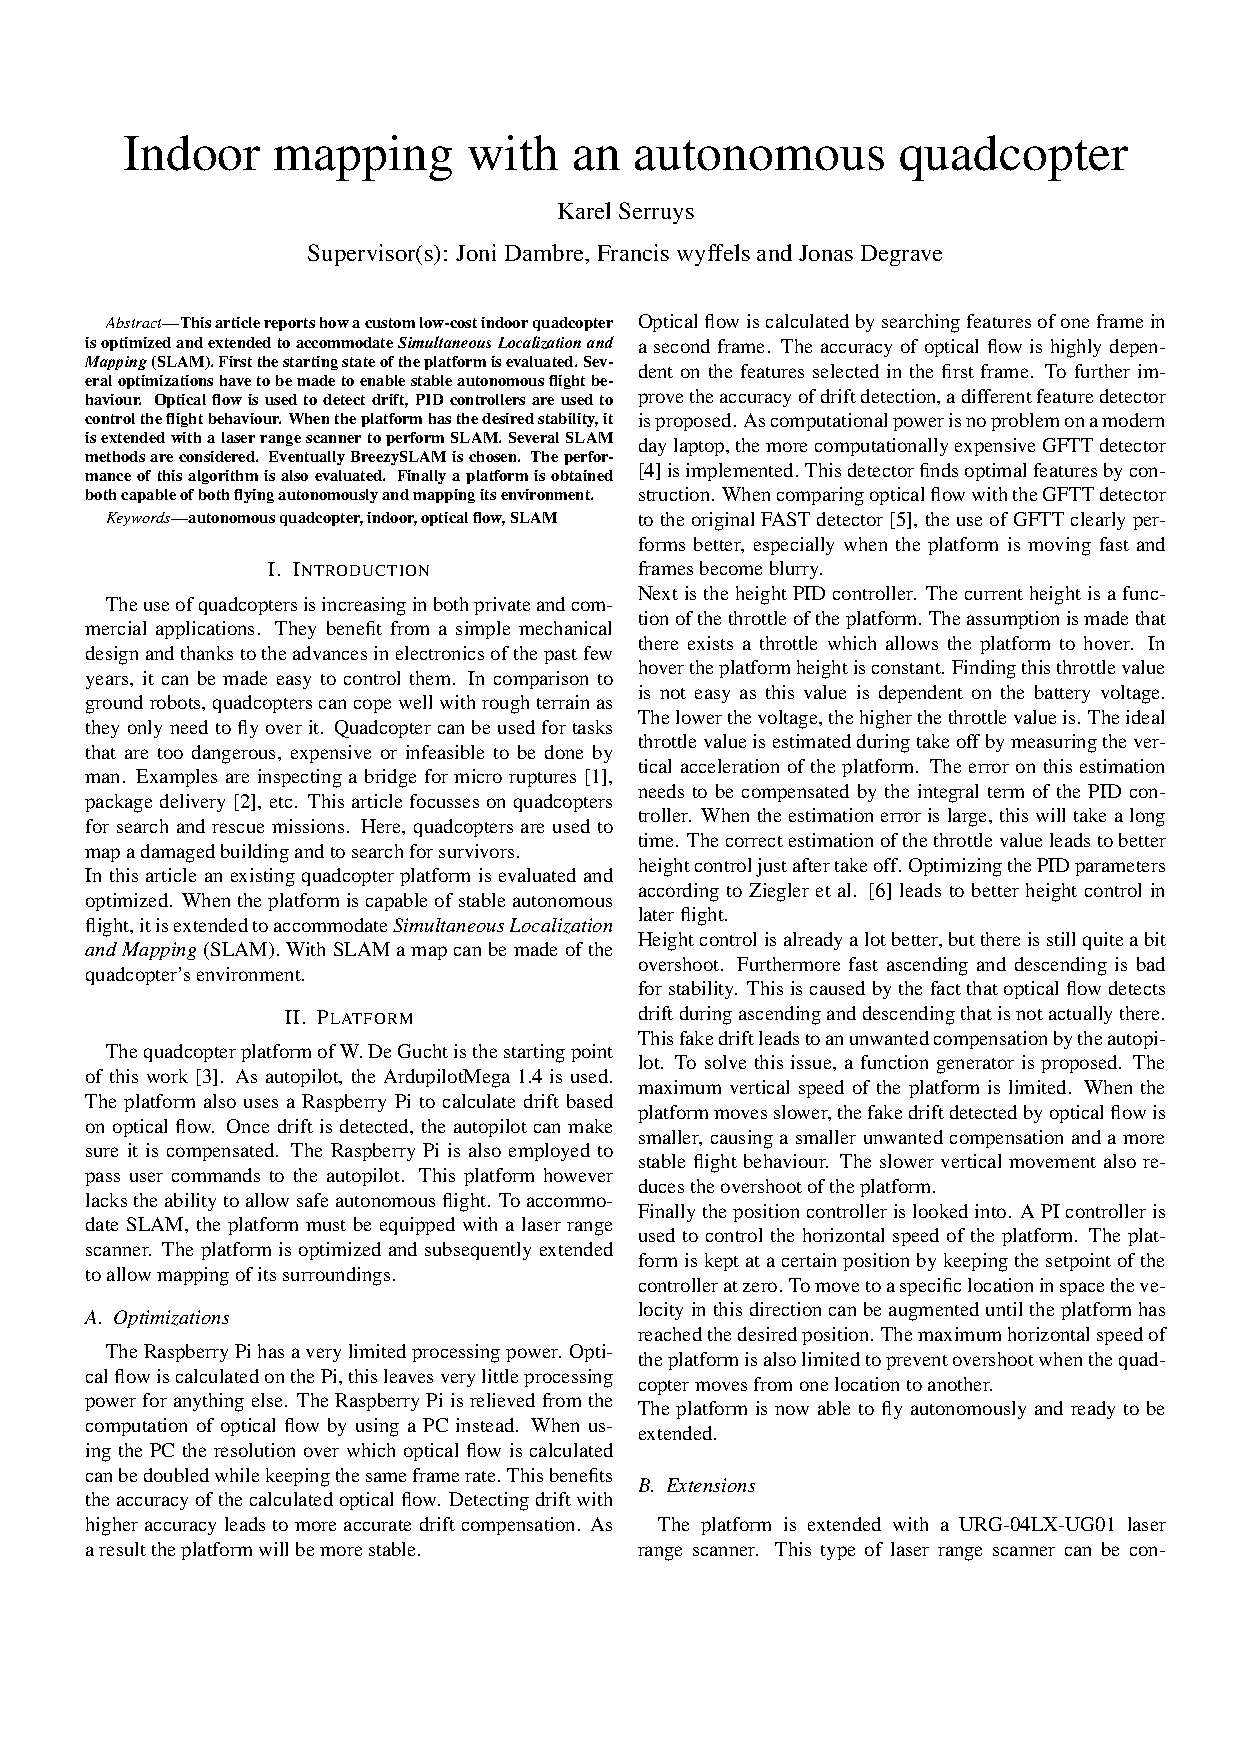
\includepdf[pages={1}]{abstract.pdf}
\includepdf[pages={2}]{abstract.pdf}
\includepdf[pages={3}]{abstract.pdf}


%inhoudsopgave
\pagestyle{fancy}
\renewcommand{\baselinestretch}{1.08} 	% De interlinie afstand wat verkleinen.
\small\normalsize                       % Nodig om de baselinestretch goed te krijgen.
\setcounter{page}{1}
\addcontentsline{tot}{chapter}{Inhoudsopgave}
\tableofcontents
\renewcommand{\baselinestretch}{1.2} 	% De interlinie afstand wat vergroten.
\small\normalsize                       % Nodig om de baselinestretch goed te krijgen.


%lijst van figuren/tabellen
\listoffigures
\listoftables
\cleardoublepage

%afkortingen en acroniemen
\chapter*{Gebruikte afkortingen}
\addcontentsline{toc}{chapter}{Gebruikte afkortingen}
\markboth{GEBRUIKTE AFKORTINGEN}{GEBRUIKTE AFKORTINGEN}
\begin{flushleft}
\renewcommand{\baselinestretch}{1.5}
\small\normalsize
\begin{longtable}{ll}
	SLAM & Simultaneous Localization and Mapping \\
	PWM & Pulse Width Modulated \\
	LiPo & Lithium-ion-Polymeer \\
	APM & Ardupilot Mega \\
	IMU & Inertial Measurement Unit \\
	RPi & Raspberry Pi \\
	SBC & Single board computer \\
	PI & Proportioneel Integrerend \\
	PID & Proportioneel Integrerend en Differenti\"erend \\
	TCP & Transmission Control Protocol \\
	GFTT & Good Features to Track \\
	FAST & Features from Accelerated Segment Test \\
	EKF & Extended Kalman Filter \\

 
\end{longtable}
\end{flushleft}

\mainmatter
% !TeX spellcheck = nl_NL
\chapter{Inleiding}

\section{Situering}\label{sec:situering}

Tegenwoordig zijn quadcopters erg populair voor zowel priv\'e als professioneel gebruik. Een belangrijke reden hiervoor is dat ze makkelijk te verkrijgen zijn en ook helemaal niet zo duur. Dit is te wijten aan hun eenvoudig ontwerp: vier armen met elk \'e\'en propeller. Door dit ontwerp is een quadcopter in staat om verticaal op te stijgen en te landen. Een nadeel is wel dat quadcopters van nature erg onstabiel zijn. De kleinste fluctuaties in motorsnelheden kunnen ervoor zorgen dat een quadcopter zijn evenwicht verliest. Om het evenwicht te herstellen moeten de snelheden van de vier motoren worden aangepast. Voor de mens is dit een te complexe taak. Daarom moet er elektronische stabiliteit voorzien worden. Hiervoor is heel wat rekenkracht nodig. Dankzij de ontwikkelingen binnen de electronica van de laatste jaren is dit in tegenstelling tot vroeger wel mogelijk. De besturing van een quadcopter wordt hierdoor erg vereenvoudigd. Een AR.Parrot is zelfs te besturen met een smartphone. Er wordt een Parrot afgebeeld in figuur \ref{fig:parrot}.

\begin{figure}[h]
	\centering
	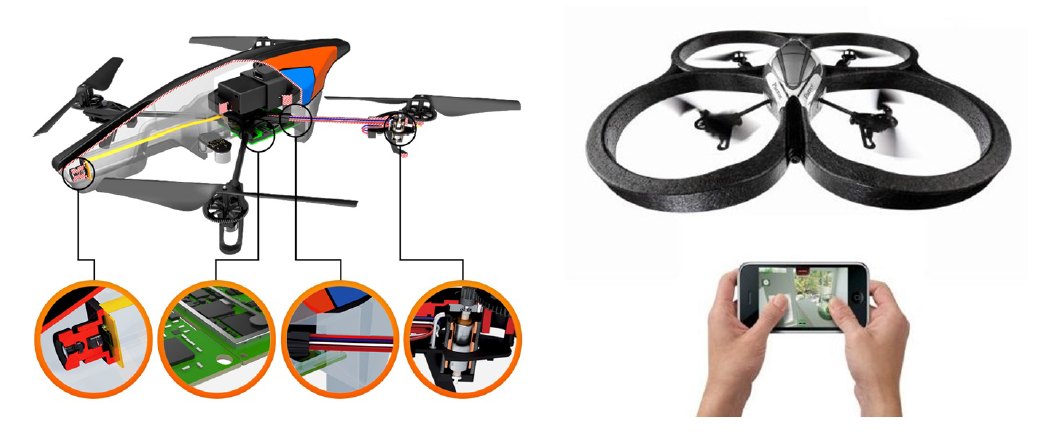
\includegraphics[width=0.6\linewidth]{parrot}
	\caption{AR.Parrot quadcopter drone die met een smartphone bestuurd kan worden.}
	\label{fig:parrot}
\end{figure}

\npar Quadcopters kunnen ingezet worden voor tal van taken. Recent kondigden de `Lokerse Feesten' bijvoorbeeld aan dat ze quadcopters willen inzetten om drank tot bij de festivalgangers te brengen die in de massa staan \cite{url:lokerse}. Uiteraard is dit geen baanbrekend idee. Er werd in het verleden reeds onderzoek gedaan naar quadcopters die in staat zijn om pakketten te leveren \cite{paper:deliveryQuad}.

% drones veiligheidsinspectie
\npar Naast het leveren van pakketten kunnen drones veiligheidsinspecties doen van hoge structuren, die moeilijk te bereiken zijn voor de mens. Hierbij wordt bijvoorbeeld rond een brug gevlogen en wordt de brug gescand op micro-scheurtjes \cite{paper:structureInspection1}\cite{paper:structureInspection2}. Om betrouwbare metingen te kunnen doen, is het belangrijk dat het gebruikte platform niet beweegt tijdens het scannen. Bovendien is het de bedoeling dat de leercurve voor het vliegen met dit platform zo laag mogelijk is. Op manier kan een persoon met weinig vliegervaring het platform toch bedienen. De input van de gebruiker wordt daarom zo laag mogelijk gehouden. Het is natuurlijk ook belangrijk dat het platform niet te pletter vliegt tegen de structuren dat het moet inspecteren. Daarom worden obstakels automatisch ontweken.

% drones mapping
\npar In deze thesis worden drones onderzocht die ingezet kunnen worden voor zogenaamde \textit{search and rescue} missies. Quadcopters zijn hiervoor beter geschikt dan grondrobots omdat ze gemakkelijk over obstakels kunnen vliegen die op de grond liggen \cite{paper:SLAMQuad2}\cite{paper:SearchRescueQuad}. Hier wil men beroep doen op drones om bijvoorbeeld een gevaarlijke site te verkennen en in kaart te brengen. Op die manier zullen reddingswerkers effici\"enter en veiliger te werk kunnen gaan. Voor het genereren van een kaart kan \textit{Simultaneous Localization and Mapping} (SLAM) gebruikt worden. SLAM bleek in het verleden al de beste oplossing voor omgevingsmapping met grondrobots. Het is dan ook niet meer dan logisch dat dezelfde techniek wordt gebruikt voor mapping en exploratie met quadcopters \cite{paper:SLAMQuad}. In \ref{sec:omgmapping} wordt reeds bestaand werk omtrent omgevingsmapping met onbemande vliegende platformen verder belicht.

\subsection{Situering van autonomie bij quadcopters} \label{sec:lcsturing}
Wanneer een quadcopter \'e\'en van de taken beschreven in \ref{sec:situering} autonoom kan uitvoeren, dan wordt het pas echt interessant. Een platform kan als autonoom beschouwd worden van zodra het staat is een taak uit te voeren zonder hulp van buitenaf. Een quadcopterplatform zal maar in staat zijn \'e\'en van de taken in \ref{sec:situering} te vervullen wanneer het stabiel vlieggedrag vertoont. Dit houdt in dat het platform gelijk welke positie in de ruimte kan aannemen en aanhouden. Hiervoor moet het platform zijn huidige positie kunnen meten. Eens gemeten, kan er ook bijgestuurd worden wanneer het platform begint af te wijken of wanneer een nieuwe positie gewenst is. Het meten van de eigen positie wordt in wat volgt \textit{lokalisatie} genoemd.

% figuur van D'Andrea
\npar Als gebruik gemaakt wordt van externe sensoren voor lokalisatie, dan spreekt men van centrale sturing. Centrale sturing voor quadcopters is een domein waar reeds veel onderzoek in verricht is.  Voor binnenshuis toepassingen worden quadcopters vaak voorzien van infrarode LED's terwijl aan het plafond een infraroodcamera gemonteerd wordt om de quadcopters te lokaliseren \cite{paper:flyingInvertedPendulum}. Buitenshuis kan GPS gebruikt worden \cite{paper:deliveryQuad}. Het is zo dat bij centrale sturing, quadcopters taken kunnen uitvoeren zonder dat iemand ze moet besturen, maar ze zijn zeker niet helemaal autonoom, want ze steunen op informatie van externe sensoren. Het belangrijkste en misschien ook wel bekendste onderzoek met quadcopters dat van centrale sturing gebruik maakt, is het werk van Andrea et al. Met behulp van centrale sturing kunnen hun quadcopters allerlei heel complexe taken verwezenlijken. Voorbeelden hiervan zijn het balanceren en doorgeven van een ge\"inverteerde pendulum \cite{paper:flyingInvertedPendulum}, het bouwen van complexe structuren \cite{paper:buildingQuad} en het uitvoeren van acrobatische bewegingen \cite{paper:multiflips}. De quadcopters zijn te zien in actie op figuur \ref{fig:quadAndrea}.

\begin{figure}[h]
	\centering
	\subfigure[Twee quadcopters die elkaar een ge\"inverteerde pendulum doorgeven.]{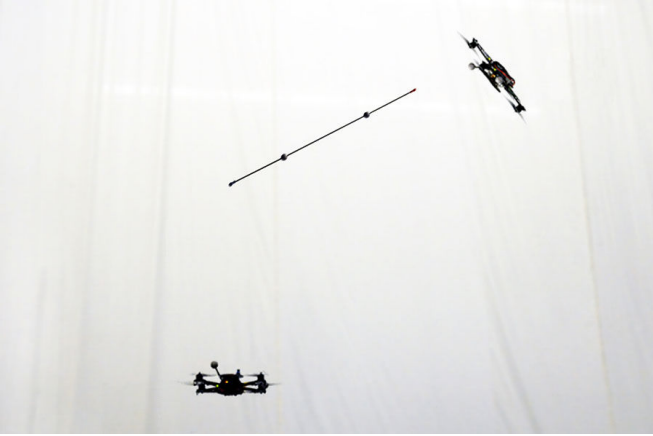
\includegraphics[width=0.48\linewidth, height=6cm]{poleAcrobatics}}
	\hspace{0.01\linewidth}
	\subfigure[Een quadcopter die een touw weeft rond twee andere touwen]{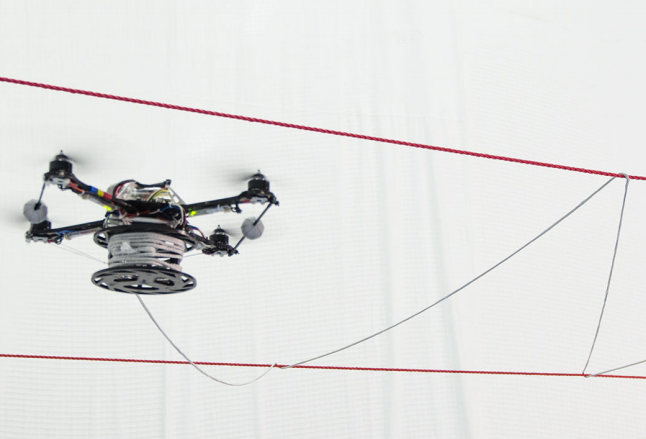
\includegraphics[width=0.48\linewidth, height=6cm]{quadbouwer}} 
	\caption{De quadcopters van Andrea et al. in actie.} \label{fig:quadAndrea}
\end{figure}

\npar Wanneer de quadcopter alle sensoren aan boord heeft, wordt gebruik gemaakt van lokale sturing. Interne sensoren zijn meestal meer onderhevig aan ruis dan externe omdat ze niet veel mogen wegen of in sommige gevallen, zoals in deze thesis, niet veel mogen kosten. Bijgevolg is lokalisatie aan de hand van lokale sturing een stuk moeilijker. In het werk van W. De Gucht wordt optical flow gebruikt, een gelijkaardige aanpak werd reeds eerder onderzocht en heeft zijn kracht bewezen \cite{paper:opticalFlowQuad}. Een andere mogelijkheid is SLAM, deze methode eist echter wel vrij veel rekenkracht. Vaak wordt dan ook een extern toestel gebruikt voor de berekeningen \cite{paper:SLAMQuad}. Het platform kan dan echter niet langer als autonoom beschouwd worden.

\subsection{Omgevingsmapping} \label{sec:omgmapping}
% belangrijkste SLAM implementaties
Binnen alle SLAM implementaties kan men drie groepen onderscheiden. Voor het verzamelen van informatie van de omgeving wordt gebruik gemaakt van ofwel een simpele camera, een laserscanner of een combinatie van die twee. Alle drie de opties hebben hun voor- en nadelen. Een camera biedt heel veel informatie, maar heeft als nadeel dat er niet rechtstreeks diepte uit gehaald kan worden. Laserscanners meten enkel diepte, hun grootste voordeel is dus ook hun grootste beperking. Een combinatie van de twee lijkt dan enkel voordelen te bieden. Dit moet natuurlijk met een korrel zout genomen worden. Het is namelijk niet evident de data van de laserscanner en de camera samen te brengen.

\begin{figure}[h]
	\centering
	\subfigure[Een map gegenereerd met een SLAM algoritme dat een laserscanner gebruikt.]{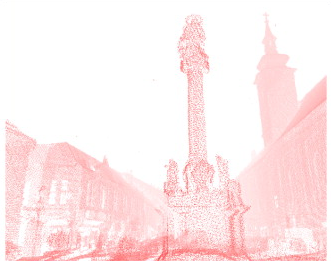
\includegraphics[width=0.45\linewidth]{3DGround2}} \label{fig:3DGrounda}
	\hspace{0.01\linewidth}
	\subfigure[Een map gegenereerd met een SLAM algoritme dat een RGB-D camera gebruikt.]{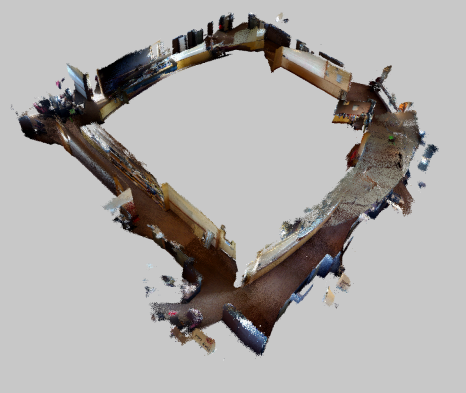
\includegraphics[width=0.45\linewidth]{3DGround}} \label{fig:3DGroundb}
	\caption{Omgevingsmappen gegenereerd door grondrobots met behulp van een 3D laserscanner(a) en met behulp van een RGB-D camera(b).}
\end{figure}

\npar Voor omgevingsmapping met grondrobots is over het algemeen genoeg rekenkracht en geheugen aanwezig om volledige 3D mappen te genereren. Deze zien er dan uit zoals in figuur \ref{fig:3DGrounda}. Om een map te bekomen als deze moet beroep gedaan worden op een vrij dure laserscanner \cite{paper:3DGround2}. Een goedkopere oplossing is een RGB-D camera gebruiken \cite{paper:3DGround}. Dit type camera registreert kleurbeelden en dieptebeelden. In figuur \ref{fig:3DGroundb} wordt een map weergegeven die met dit soort camera werd bekomen.

\npar Wanneer een quadcopter gebruikt wordt, zijn de opties een stuk beperkter. Ten eerste is er de beperkte last die ze kunnen dragen. De gebruikte scanner of camera mag niet te zwaar zijn. Ten tweede beschikt het platform over een beperkte rekenkracht. Het is dan ook zo dat vaak een extern toestel gebruikt wordt voor het genereren van de map. De quadcopter staat dan enkel in voor het verzamelen van de informatie. De thesis van J. Nyman  gebruikt deze aanpak. \textit{Parallel Tracking And Mapping} (PTAM) werd ge\"implementeerd met behulp van een camera \cite{thesis:jens}. Het resultaat is te zien in figuur \ref{fig:PTAM}. In het werk van S. Shen et al. wordt een laserscanner gebruikt in combinatie met een RGB-D camera \cite{paper:3DQuad} . Bovendien gebeuren alle berekeningen aan boord van het platform. Het resultaat is te zien in figuur \ref{fig:3DSlam}. De lezer kan al vermoeden dat de gebruikte hardware voor deze aanpak een heel stuk kostelijker is dan de hardware die J. Nyman gebruikte. Er moet nog opgemerkt worden dat het werk van J. Nyman wel een 3D map genereert, maar die is eigenlijk gebaseerd op 2D data.

%figuur SLAM Jens
\begin{figure}[h]
	\centering
	\subfigure[Een map gegenereerd met de PTAM implementatie van J. Nyman. Het PTAM algoritme maakt gebruik van een camera.]{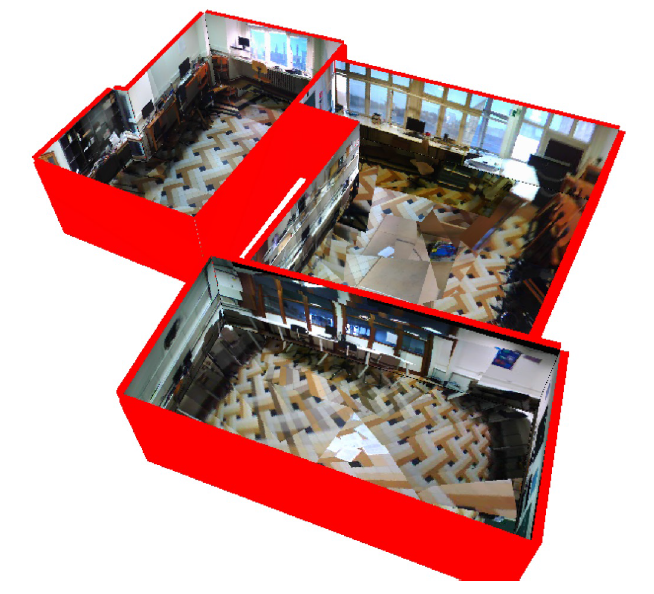
\includegraphics[width=0.45\linewidth]{PTAM}\label{fig:PTAM}}
	\hspace{0.01\linewidth}
	\subfigure[Een map gegenereerd met het SLAM algoritme geschreven door S. Shen et al. dat gebruik maakt van een RGB-D camera en een laserscanner]{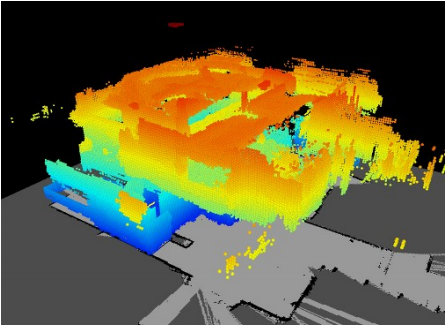
\includegraphics[width=0.45\linewidth]{3DSlam}\label{fig:3DSlam}}
	\caption{Omgevingsmappen gegenereerd door quadcopters met behulp van een camera(a) en met behulp van een laserscanner en een RGB-D camera (b).}
\end{figure}


\section{Probleemstelling}
Er moet een goedkoop \textbf{autonoom platform} gebouwd worden dat zichzelf in evenwicht houdt met behulp van \textbf{lokale sturing}. Dit wil zeggen dat het platform een vaste positie moet kunnen aanhouden zonder weg te driften. Hiervoor mag enkel gebruik gemaakt worden van interne sensoren.

\npar Daarnaast moet het platform geschikt zijn voor \textbf{omgevingsmapping}. Hiervoor moet gebruik gemaakt worden van een laserscanner in combinatie met een SLAM algoritme. Indien nodig kan ook de odometrie van het platform gebruikt worden om een nauwkeurigere omgevingsmap te genereren.

\section{Aanpak}
Om de lezer op de hoogte te brengen van de specificaties en de werking van het platform bij aanvang van deze thesis, wordt hier eerst een hoofdstuk aan besteed. Het is de bedoeling om de quadcopter volledig op zichzelf een onbekende ruimte te laten verkennen. Om geen gevaar te vormen voor zichzelf of voor zijn omgeving, moet het platform voldoende stabiel zijn. Daarom worden in het derde hoofdstuk van deze thesis een aantal optimalisaties voorgesteld om het vlieggedrag van het huidige platform te verbeteren. In hoofdstuk vier wordt er op zoek gegaan naar een geschikt SLAM algoritme om het dan in hoofdstuk vijf te integreren in het platform.

% !TeX spellcheck = nl_NL
 \chapter{Quadcopter platform}

%figuur aanvang thesis

Deze thesis is het vervolg op de thesis van W. De Gucht \cite{thesis:wouter}. In dit hoofdstuk wordt de situatie geschetst zoals die was bij de aanvang van deze thesis. Eerst wordt wat terminologie aangehaald, dan wordt de hardware van het platform overlopen en vervolgens wordt de functie van de belangrijkste softwareblokken belicht.

\section{Terminologie}

\begin{figure}[h]
	\centering
	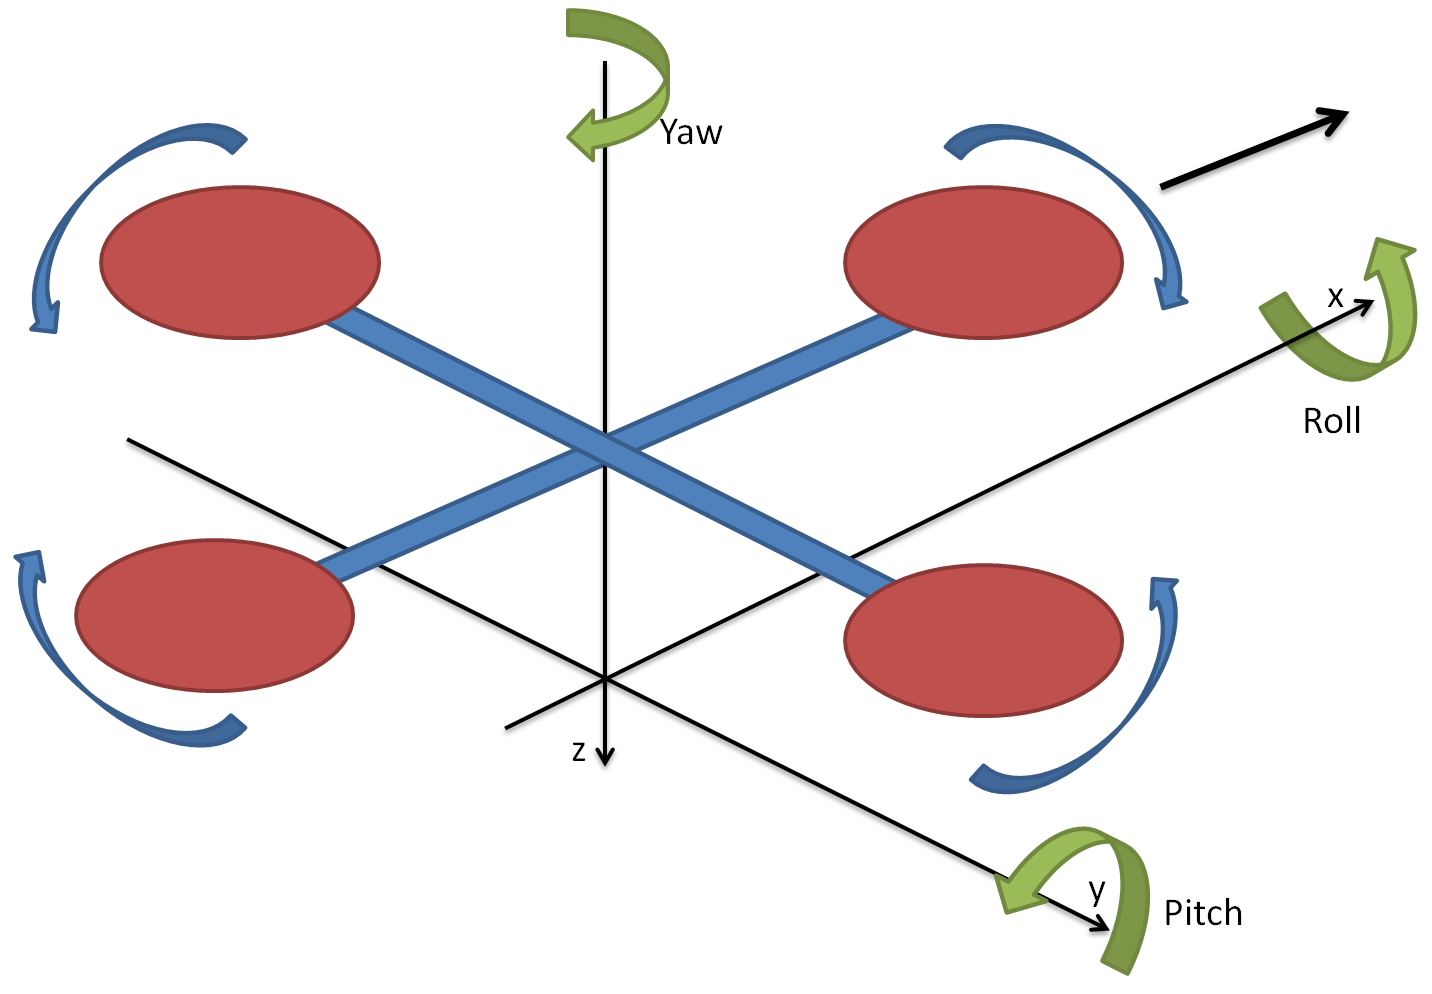
\includegraphics[width=0.6\linewidth]{yaw_pitch_roll}
	\caption{Schematische voorstelling van een quadcopter waarop het gebruikte assenstelsel en roll, pitch en yaw zijn aangeduid.}\label{fig:yaw_pitch_roll}
\end{figure}
\noindent Er wordt een rechtshandig assenstelsel gehanteerd, te zien op figuur \ref{fig:yaw_pitch_roll}, waarbij de z-as naar de grond is gericht. Binnen de aerodynamica wordt gebruik gemaakt van de hoeken \textit{roll}, \textit{pitch} en \textit{yaw} om de positie ten opzichte van de grond van een vliegend toestel uit te drukken. De namen van die hoeken worden ook in deze thesis gehanteerd. De roll is de rotatie rond de x-as, de pitch rond de y-as en de yaw rond de z-as. De snelheid waarmee een motor draait, krijgt de naam \textit{throttle}. Yaw, pitch, roll en de throttle van de vier motoren vormen samen het \textit{gedrag} van de quadcopter.

\section{Hardware}
In deze sectie komt de hardware van het platform aan bod. Er wordt een onderverdeling gemaakt op basis van de functie van de componenten. Het eerste deel, de quadcopterbasis, bestaat uit het frame, de motoren, de \textit{Electronic Speed Controllers} (ESC's) en de batterij. Het tweede deel, de quadcoptersturing omvat de hardware componenten die instaan voor het regelen van het vlieggedrag van het platform: de \textit{Raspberry Pi} (RPi) en de \textit{Ardupilot Mega} (APM). Alle componenten (behalve het frame) worden weergegeven op figuur \ref{fig:hardware}.

\begin{figure}[h]
	\centering
	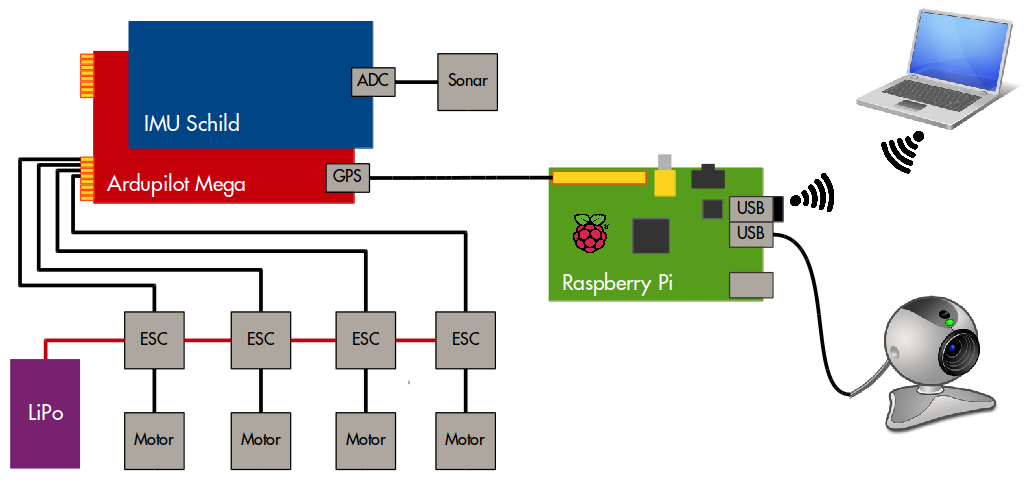
\includegraphics[width=0.9\linewidth]{hardware_whole}
	\caption{De hardware van het platform, schematisch voorgesteld.}
	\label{fig:hardware}
\end{figure}

\subsection{Quadcopterbasis}
Een overzicht van de quadcopterbasis wordt afgebeeld in figuur \ref{fig:quadbasis}. Alle onderdelen behalve de batterij worden weergegeven. Meestal wordt de batterij ergens onderaan of bovenaan het platform bevestigd net voor het vliegen.

\begin{figure}[ht]
	\centering
	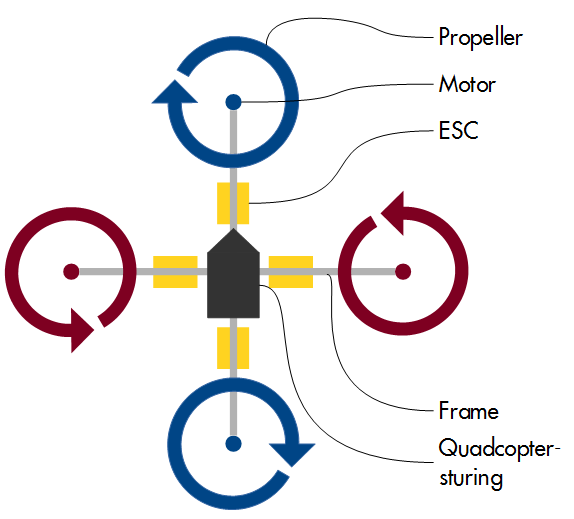
\includegraphics[width=0.50\linewidth]{quad}
	\caption{Overzicht van de quadcopterbasis.}
	\label{fig:quadbasis}
\end{figure}


\subsubsection{Frame}
De basis van de quadcopter is een \textit{plus-vormig} frame zoals te zien is in figuur \ref{fig:quadbasis}. In het midden van het frame is een ruimte voorzien voor het bevestigen van de elektronica die nodig is voor de sturing van het platform. Zoals het hoort staat op iedere arm een motor.

\subsubsection{Motoren}
Er wordt gebruik gemaakt van brushless DC motoren. Deze motoren maken geen fysisch contact om de ompoling in de kern te cre\"eren. Hierdoor is dit type motor erg efficient. De motoren vragen een maximale stroom van \SI{10}{A}.

\npar Aan iedere motor is een propeller bevestigd. Twee ervan moeten draaien in wijzerzin, de andere twee in tegenwijzerzin. De draairichting van de propellers is aangeduid op figuur \ref{fig:quadbasis}. Moesten alle vier de rotoren in dezelfde richting draaien, dan zou de quadcopter voortdurend rond zijn as roteren. De propellers die draaien in wijzerzin compenseren dus de draaiimpuls van die in tegenwijzerzin (omgekeerd geldt hetzelfde).

\subsubsection{ESC's}
Op alle vier de armen is een \textit{Electronic Speed Controller} (ESC) bevestigd. Het zijn \SI{20}{A} ESC's. Ze kunnen dus zeker genoeg stroom leveren om de motoren op hun snelst te laten werken.

\npar De ESC's moeten een \textit{Pulse Width Modulated} (PWM) signaal omzetten in een driefasig stroomsignaal. Dit laatste signaal zorgt ervoor dat de spoelen van de motoren afwisselend stroom krijgen en de motoren dus aan het draaien gaan. De duty cycle van het PWM signaal bepaalt de frequentie van het driefasig signaal dat een motor ontvangt. Hoe hoger de duty cycle, hoe hoger de frequentie van het driefasig signaal en hoe sneller de motor zal draaien.

\subsubsection{Batterij}
Om het platform te voeden wordt een 1000\,mAh lithium-ion-polymeer (LiPo) batterij gebruikt. Deze soort batterij kan indien nodig de \SI{40}{A} leveren die de motoren nodig hebben als ze op hun snelst werken.

\subsection{Quadcoptersturing} \label{sec:quadcoptersturing}
De sturing van het platform is onder te verdelen in twee delen. Op de eerste plaats is er de \textit{Ardupilot Mega} (APM) met bijhorend \textit{Inertial Measurements Unit} (IMU) schild. Deze twee bordjes staan in voor de controle van het vlieggedrag van de quadcopter. Op de tweede plaats is er de \textit{Raspberry Pi} (RPi). Deze \textit{single board computer} (SBC) wordt gebruikt om het gewenste vlieggedrag door te geven aan de APM. Bovendien wordt de RPi ook gebruikt om de snelheid van het platform te berekenen. Die berekende snelheid wordt door de APM gebruikt om de quadcopter in de ruimte te lokaliseren en eventuele drift ten opzichte van de gewenste positie te compenseren.

\subsubsection{Quadcopter sturen}
Een quadcopter kan op eenvoudige manier gestuurd worden. Om naar links, rechts, voor en achter te vliegen, kan gewoon de snelheid van \'e\'en motor aangepast worden. Figuur \ref{fig:navigate} (links) geeft dit weer een voorwaartse beweging. Door de snelheid van de achterste motor op te drijven zal de pitch verkleinen. De quadcopter kantelt naar voor. De propellers stuwen lucht nu deels naar achter. Als reactie vliegt de quadcopter naar voor. Door rotoren met dezelfde draaizin even te versnellen kan de yaw veranderd worden. Dit omdat de torsie in die draaizin dan niet wordt opgehoffen door de motoren met de andere draaizin. Figuur \ref{fig:navigate} (rechts) geeft dit weer.

\begin{figure}
	\begin{center}
		\subfigure{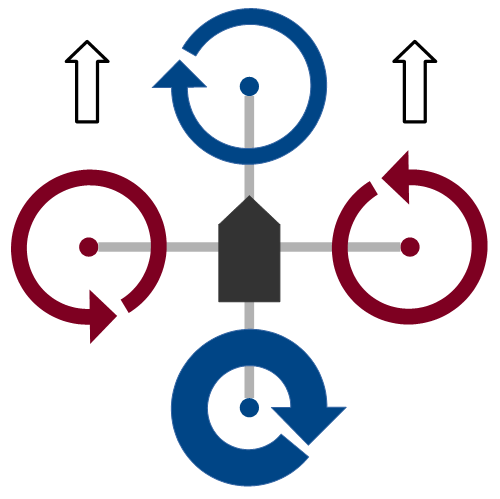
\includegraphics[width=0.40\linewidth]{navigate2}}
		\hspace*{0.1\linewidth}
		\subfigure{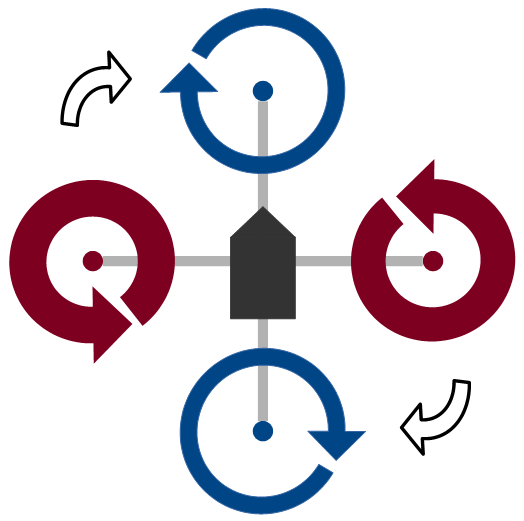
\includegraphics[width=0.40\linewidth]{navigate1}}
	\end{center}
	\centering
	\caption{Om een quadcopter vooruit te laten vliegen, moet de throttle van de achterste motor opgedreven worden (links). Om een quadcopter te laten roteren om de z-as moet de throttle van de rotoren in wijzerzin verschillen van die in tegenwijzerzin (rechts).}
	\label{fig:navigate}
\end{figure}

\subsubsection{Ardupilot Mega en IMU schild}
De APM, afgebeeld op figuur \ref{fig:APMIMU} (links), is het brein van de quadcopter. Het bordje heeft twee microcontrollers. De ATmega2560 is hiervan de belangrijkste. Het is een 8-bit microcontroller die alle inkomende data ontvangt en verwerkt. Hier wordt het gedrag bijgestuurd om het gewenste vlieggedrag te bekomen. De controlesignalen die bestemd zijn voor de motoren gaan naar de tweede microcontroller, de ATmega328. Deze controller moet ervoor zorgen dat deze signalen omgezet worden in PWM signalen. Dankzij deze tweede component, wordt de ATmega2560 minder belast en blijft er meer rekenkracht over voor berekeningen met betrekking tot stabilisatie.

\begin{figure}
	\centering
	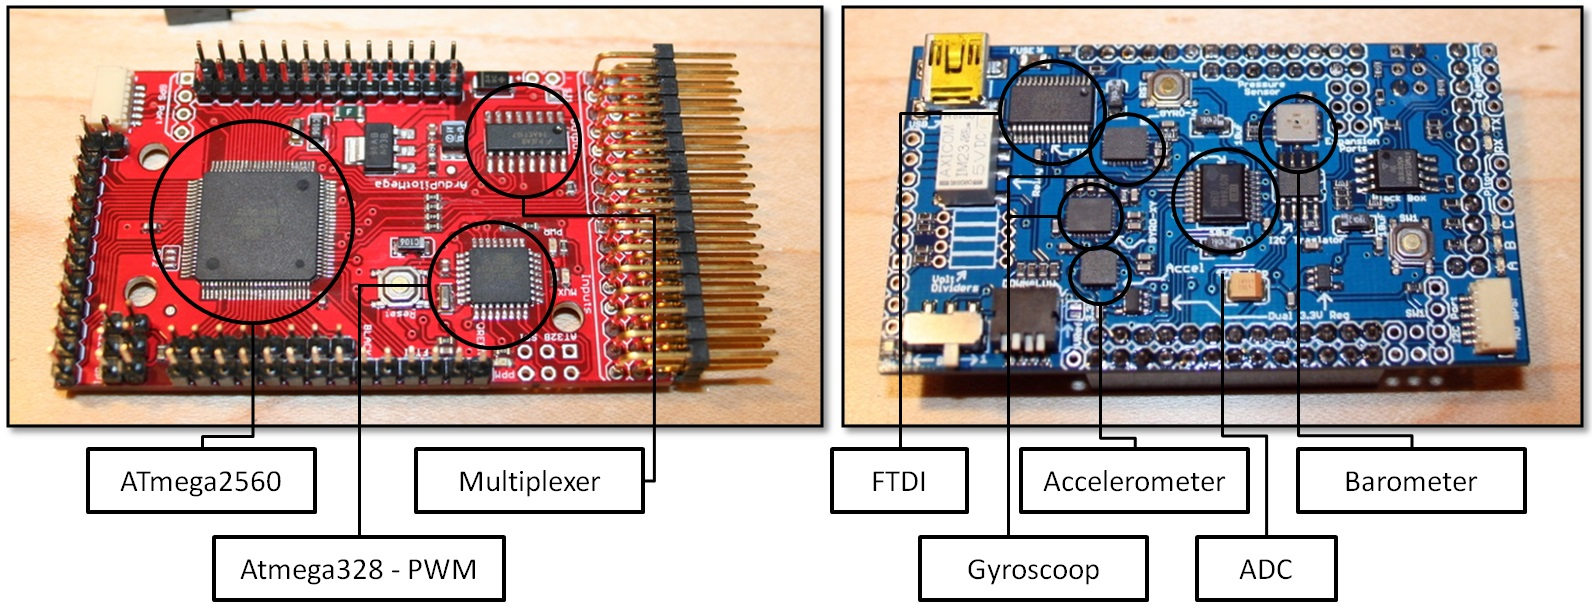
\includegraphics[width=0.8\linewidth]{APMIMU}
	\caption{De Ardupilot Mega(links) en het Inertial Measurements Unit schild(rechts) met hun belangrijkste componenten aangeduid op de figuur.}
	\label{fig:APMIMU}
\end{figure}

\npar De APM ontvangt data van de RPi via een seri\"ele verbinding. Deze verbinding is aangesloten op de APM waar normaal een GPS ontvanger moet komen. De APM kan ook sensoren uitlezen die op het IMU schild aanwezig zijn.

\npar Het IMU schild, ook weergegeven in figuur \ref{fig:APMIMU} (rechts),  beschikt over een gyrscoop waarmee de hoeksnelheid ten op zichte van alle assen kan gemeten worden. Er is ook een tri-axiale accelerometer die de versnelling in drie richtingen kan meten, in de richting van de x-as, y-as en de z-as. Bovendien wordt er ook een sonar verbonden die de hoogte van de quadcopter meet ten opzichte van de grond.

\subsubsection{Raspberry Pi}
De Raspberry Pi is \'e\'en van de bekendste SBC's op de markt. Omdat er een linux installatie op kan draaien is het eenvoudig om randapparatuur aan te sluiten. De RPi wordt voorzien van een camera die als input kan dienen voor optical flow. Voor communicatie met de APM is er zoals hierboven vermeld een seri\"ele verbinding voorzien. Er is ook een WiFi-dongle aanwezig om communicatie met de PC mogelijk te maken. De RPi met bijhorende randapperaten staat ook afgebeeld op figuur \ref{fig:hardware}.

\npar In de loop van de thesis werd de RPi\,2 uitgebracht. Deze SBC is veel krachtiger dan zijn oudere variant. Ter vergelijking worden de specificaties van de RPi\,1 en de RPi\,2 weergegeven in tabel \ref{table:RP1vsRPI2}. Naar het einde van deze thesis toe zal het gebruik van de nieuwe versie noodzakelijk worden.

\begin{table}[h]
	\caption{Vergelijking tussen aanvankelijk gebruikte RPi en het nieuwste model op de markt.} \label{table:RP1vsRPI2}
	\centering
	\begin{tabular}{lcc}
		\cr
		\hline
		& Raspberry Pi Model B & Raspberry Pi 2 Model B \\
		\hline
		CPU & 700 MHz & 900 MHz (Quadcore) \\
		RAM & 512 MB & 1 GB \\
		USB 2.0 poorten & 2 & 4 \\
		Stroomvoorziening & 5V & 5V \\
		\hline
	\end{tabular}
\end{table}

\section{Software}
In deze sectie worden alle aspecten van de quadcoptersturing uitgelegd. Hoe de quadcopter stabiel wordt gehouden en hoe er met het platform wordt gecommuniceerd. Zoals al eerder werd aangehaald, zijn de APM en de RPi de hardware componenten die instaan voor de sturing. Hun functie binnen het geheel komt hieronder ook in die volgorde aan bod.

\subsection{Ardupilot Mega} \label{sec:softAPM}
Binnen de APM kan er opgesplitst worden in twee delen. De software die instaat voor stabilisatie draait binnen de APM controlelus. Daarnaast is er ook nog de gebruikerlus. Hierin kan het gedrag van de quadcopter geprogrammeerd worden om uiteindelijk een autonoom platform te bekomen. De volledige architectuur van de APM wordt weergegeven in figuur \ref{fig:APMsoftware}.

\begin{figure}[h]
	\centering
	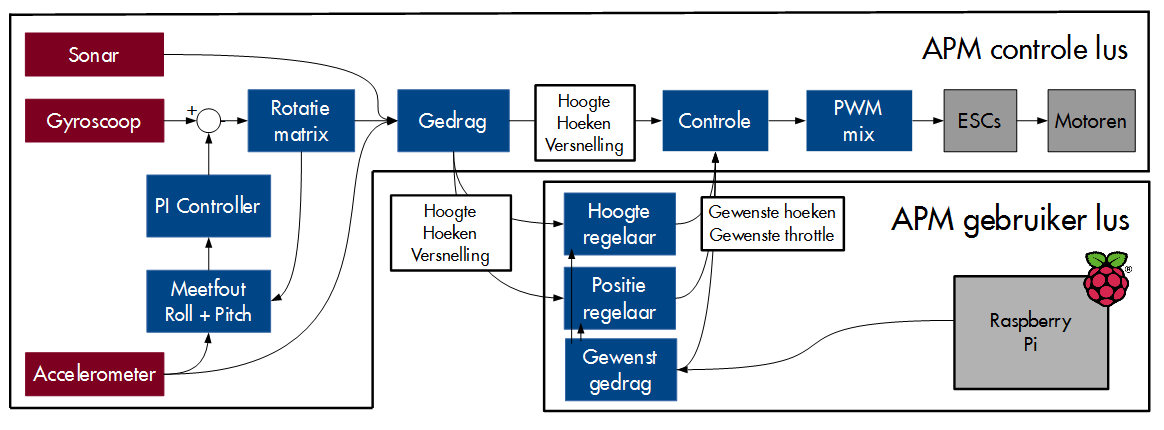
\includegraphics[width=\linewidth]{APMsoftware}
	\caption{Architectuur van de Ardupilot Mega.}
	\label{fig:APMsoftware}
\end{figure}

\subsubsection{Ardupilot controlelus}
In de rotatiematrix worden de hoeken ten opzichte van het referentiestelsel bijgehouden. Deze matrix wordt constant ge\"updatet met de hoeksnelheden gemeten door de gyroscoop. De rotatiematrix moet orthogonaal zijn. De meetfout van de gyroscoop moet dus gecompenseerd worden. Dit gebeurt door renormalisatie toe te passen. De fout op de hoeken wordt hier gecompenseerd door ervoor te zorgen dat de rotatiematrix opnieuw orthogonaal wordt.

\npar De rotatiematrix is nu reeds vrij betrouwbaar. Er zit wel nog een zekere drift op. Om deze drift te compenseren wordt accelerometerdata gebruikt. De zwaartekracht kan gemeten worden, deze is evenwijdig met de z-as van het referentiestelsel. Hieruit kan dan de meetfout op pitch en roll gehaald worden. De meetfout wordt dan met een PI-regelaar teruggevoerd naar de rotatiematrix.

\npar De hoogte van het platform gemeten door de sonar, de hoeken berekend door de rotatiematrix en de accelerometerdata gemeten door de accelerometers worden doorgegeven aan het gedrag. In het gedrag kan dus de huidige toestand van het platform terug gevonden worden. De huidige toestand wordt in de gebruikerlus gebruikt om hoogte en positie van het platform te regelen. Het gedrag wordt ook naar de controle gestuurd.

\npar In de controle wordt het gedrag gebruikt om de corrigerende acties te berekenen die nodig zijn om de quadcopter stabiel te houden. Daarnaast neemt de controle ook het gewenste gedrag in acht. De snelheid waarmee iedere motor moet draaien wordt berekend. Het resultaat wordt dan doorgegeven naar de PWM mixer en omgezet in PWM signalen. De ESC's maken van die PWM signalen de driefasige stroomsignalen waarmee de motoren bestuurd worden.

\subsubsection{Ardupilot gebruikerlus}
De gebruikerlus neemt als ingang het gedrag van de quadcopter. Zoals reeds werd vermeld bevat dit gedrag de hoogte, de hoeken ten opzichte van het referentiestelsel en de versnellingen in alle richtingen. Daarnaast wordt ook optical flow data ontvangen van de RPi.

\npar De hoogte PID-regelaar neemt de hoogte als input. De gewenste hoogte kan via de RPi worden ingesteld. De huidige hoogte wordt gecorrigeerd door de gewenste throttle aan te passen.

\npar Een positie PID-regelaar neemt de hoeken, de versnelling en de optical flow data afkomstig van de RPi als input. Met deze informatie kan de exacte locatie van de quadcopter berekend worden. Ook hier wordt de exacte positie vergeleken met de setpoint ingesteld via de RPi. De positie kan gecorrigeerd worden door roll en pitch bij aan te passen. Als het platform van zijn gewenste positie wegdrift, dan moet deze PID-regelaar die drift tegenwerken.

\npar Het effectief berekenen van de locatie van het platform verdient nog een klein woordje uitleg. De optical flow data die gebruikt wordt voor de berekening van de locatie van het platform, bevat de optische snelheden $(OF_x)_{ongecomp.}$ en $(OF_y)_{ongecomp.}$ van het platform, gemeten over twee camerabeelden. Om hieruit de effectieve snelheid af te leiden moeten nog een aantal berekeningen gebeuren. Om de correcte snelheid af te leiden moet rekening gehouden worden met de roll, de pitch en de hoogte van de quadcopter. Dit wordt verduidelijkt door figuur \ref{fig:invloed}.

\begin{figure}[h]
	\centering
	\subfigure[Invloed van roll en pitch op optical flow snelheid.]{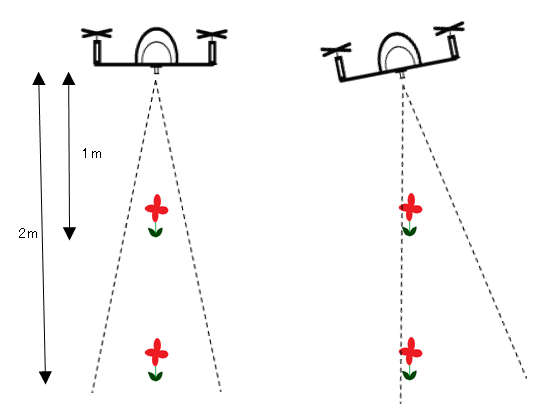
\includegraphics[width=0.48\linewidth]{invloedhoek}}
	\hspace{0.01\linewidth}
	\subfigure[Invloed van hoogte op optical flow snelheid.]{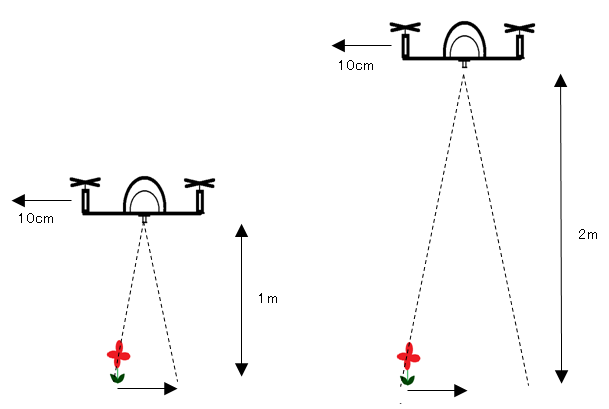
\includegraphics[width=0.48\linewidth]{invloedhoogte}}
	\caption{Bij het omzetten van optical flow data naar een effectieve snelheid moet rekening gehouden worden met roll en pitch(a) en met de hoogte(b) van het platform.} \label{fig:invloed}
\end{figure}

\npar Ten eerste moet het verschil in roll en pitch tussen de twee cameraopnames gecompenseerd worden. Als dit niet wordt gedaan, dan klopt de door optical flow gedetecteerde snelheid niet. Stel dat het platform een beetje kantelt, maar toch op dezelfde positie in de lucht blijft hangen. Er zal toch optical flow gedetecteerd worden, terwijl het platform zich eigenlijk niet verplaatst. Dit probleem wordt afgebeeld op figuur \ref{fig:invloed}(a). Formules \eqref{eq:comproll} en \eqref{eq:comppitch} kunnen gebruikt worden om de ontvangen optische snelheden te compenseren met $\omega_{roll}$ en $\omega_{pitch}$, de roll- en pitchhoeksnelheid \cite{thesis:wouter}. Nu geweten is hoe de optische snelheid gecompenseerd moeten worden, moet het goeie moment voor deze compensatie nog worden uitgekozen. Omdat de optical flow data van de RPi moet komen, zit er een zekere delay op. Deze delay blijkt twee tijdstappen groot te zijn. Hierbij is \'e\'en tijdstap de tijd tussen twee ontvangen optical flow vectoren.

\begin{equation}
OF_x = (OF_x)_{ongecomp.} - \omega_{pitch} \cdot \frac{R_x}{K_x}
\label{eq:comproll}
\end{equation}
\begin{equation}
OF_y = (OF_y)_{ongecomp.} - \omega_{roll} \cdot \frac{R_y}{K_y}
\label{eq:comppitch}
\end{equation}

\npar Vervolgens moet de snelheid die nu nog uitgedrukt is in pixels per seconde omgezet worden in meter per seconde. De hoogte $h$, de kijkhoeken $K_x$ en $K_y$ en de resolutie $R_x$x$R_y$ van de gebruikte camera zijn gekend. Na enkele simpele goniometrische berekeningen blijkt dat forumles \eqref{eq:vx} en \eqref{eq:vy} de snelheid in meter per seconde geven \cite{thesis:wouter}.

\begin{equation}
v_x = OF_x \cdot \frac{2 \cdot h \cdot \tan(K_x/2)}{R_x}
\label{eq:vx}
\end{equation}
\begin{equation}
v_y = OF_y \cdot \frac{2 \cdot h \cdot \tan(K_y/2)}{R_y}
\label{eq:vy}
\end{equation}

\subsection{Raspberry Pi} \label{sec:softRPi}

Figuur \ref{fig:RPIloop} geeft de architectuur van de RPi weer. Optical flow wordt berekend in \textit{OpticalFlow.cpp} en doorgestuurd naar het serieel model. $Keyboard.py$ kijkt naar input van de gebruiker en plaatst die in de wachtrij van het serieel model. Het serieel model, $SerialModel.py$, beheert het verkeer tussen de APM en de verschillende processen op de RPi.

\begin{figure}[h]
	\centering
	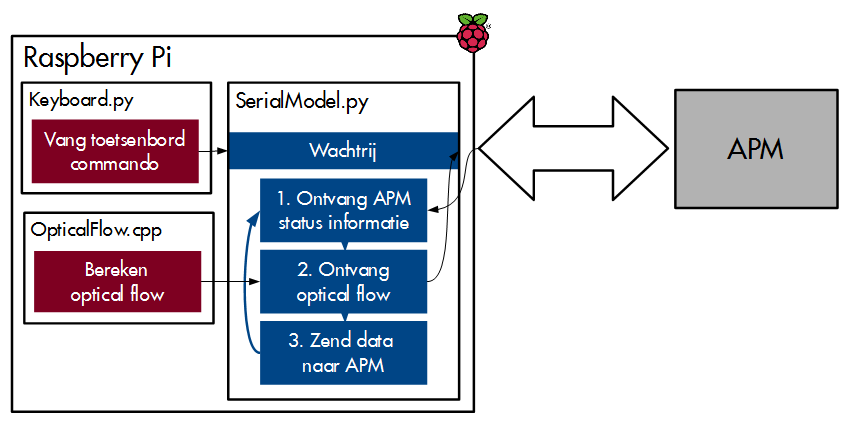
\includegraphics[width=0.8\linewidth]{RPIloop.png}
	\caption{Architectuur van de Raspberry Pi.}
	\label{fig:RPIloop}
\end{figure}

\npar De Raspberry Pi vervult hiermee vier taken, hieronder gerangschikt met dalende prioriteit:
\begin{itemize}
\item[1.] Optical flow berekenen
\item[2.] Optical flow data verzenden naar APM.
\item[3.] Uitprinten of opslaan van de statusinformatie afkomstig van APM.
\item[4.] Commando's van de computer verzenden naar APM.
\end{itemize}

\noindent Taak 1: het berekenen van optical flow, het algoritme voor deze berekening wordt uitgelegd in \ref{sec:OptFlow}. De APM verwacht de optische snelheid van het platform. De optische snelheid wordt telkens doorgestuurd naar de lus van het serieel model via een \textit{non-blocking send}. Op die manier kan het programma onmiddellijk aan de volgende berekening beginnen. In het serieel model wordt gebruik gemaakt van een \textit{blocking receive} bij het ontvangen van optical flow data. Op die manier wordt verzekerd dat de data doorgestuurd wordt naar de APM van zodra ze beschikbaar is.

\npar In de lus van het serieel model worden taken 2 tot 4 voortdurend uitgevoerd. Als er commando's worden ontvangen van de computer, worden die telkens achteraan in de wachtrij toegevoegd. Wanneer er optical flow data beschikbaar is, wordt die telkens vooraan in de wachtrij gezet en wordt de hele wachtrij verzonden. De mogelijke commando's en hun betekenis worden opgelijst in tabel \ref{table:oldcom}.

\begin{table}[h]
	\caption{Nieuwe commando's om het vlieggedrag te be\"invloeden.}\label{table:oldcom}
	\centering
	\begin{tabular}{cp{.3\linewidth}cp{.3\linewidth}}
		\cr
		\hline
		Commando & Betekenis & Commando & Betekenis \\
		\hline
		z & Verhoog pitch & s & Verlaag pitch\\
		q & Verhoog roll & d & Verlaag roll \\
		w & Verhoog yaw & x & Verlaag yaw \\
		a (auto) & Verhoog gewenste hoogte & e (auto) & Verlaag gewenste hoogte \\
		a (manueel) & Verhoog throttle & e (manueel) & Verlaag throttle\\
		c & Ga naar manuele modus & v & Ga naar manuele modus \\	
		r & Leg motoren aan & t & Schakel motoren uit \\	
		f & Print quadcopterstatus & & \\
		\hline				
	\end{tabular}
\end{table}

\npar Taak 3 spreekt voor zich, wanneer de APM statusinformatie ter beschikking stelt, wordt deze geprint en eventueel ook opgeslagen. Deze statusinformatie is heel handig voor het debuggen van de APM software. De statusinformatie kan ook gebruikt worden om het vlieggedrag na een vlucht visueel voor te stellen.

%sectie over de werking en implementatie van optical flow!!
\subsection{Optical flow} \label{sec:OptFlow}
Het belang van optical flow werd reeds aangewezen in \ref{sec:softAPM}. Het gebruikte algoritme voor het berekenen van optical flow snelheden wordt uit de doeken gedaan aan de hand van figuur \ref{fig:algOptFlow}.
%figuur met optical flow algoritme
\begin{figure}[h]
	\centering
	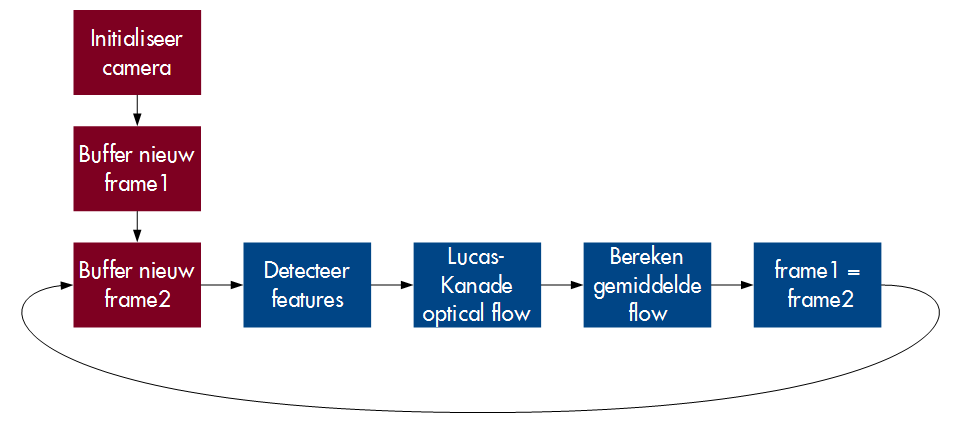
\includegraphics[width=0.8\linewidth]{algOpticalFlow}
	\caption{Het optical flow algoritme wordt in deze figuur grafisch voorgesteld.} \label{fig:algOptFlow}
\end{figure}

\npar Om te beginnen wordt de camera ge\"initialiseerd. Vervolgens worden de eerste twee frames in een buffer opgeslagen. Nu is alle nodige data beschikbaar om de eerste optical flow snelheidsvector te berekenen. 

\npar In het eerste frame wordt met de FAST detector \cite{paper:FAST} gezocht naar goede features. De werking van deze detector wordt in \ref{sec:FAST} kort uitgelegd. Eens features geselecteerd zijn, moeten die gezocht worden in het tweede frame. Wanneer de verplaatsing van iedere feature over de twee frames gekend is, wordt de gemiddelde optische verplaatsing berekend. Zoals reeds vermeld verwacht de PID-regelaar van de APM optische snelheden. De gemiddelde verplaatsing moet dus enkel nog gedeeld worden door de tijd tussen de twee frames. Eens de optical flow data is verstuurd kan er overgegaan worden naar het volgende frame. Het eerste frame wordt vervangen door het tweede, een nieuw frame wordt gebufferd en de hierboven beschreven stappen herhalen zich.

\npar Het zoeken van de optical flow tussen twee frames gebeurt zoals beschreven werd door J.Y. Bouguet in ``Pyramidal Implementation of the Affine Lucas Kanade Feature Tracker" \cite{paper:PyrLK}. Deze paper stelt een effici\"ente manier voor om de feature tracker voorgesteld door Lucas en Kanade \cite{paper:LK} te implementeren. De methode maakt gebruik van beeldpiramides. De geselecteerde features van het eerste frame worden eerst gezocht in een lage resolutie-kopie van het tweede frame. Wanneer een match gevonden wordt, moet enkel nog in de buurt deze match gezocht worden in de hogere resolutie-kopi\"en. Dit zorgt ervoor dat het zoeken van features in het tweede frame veel sneller gaat dan wanneer rechtstreeks in het oorspronkelijke frame gezocht zou worden.

\npar Zowel de FAST detector en de gebruikte optical flow implementatie zijn beschikbaar in de OpenCV bibliotheek \cite{url:opencv}. Het is dan ook niet meer dan logisch dat deze bibliotheek wordt gebruikt.

\section{Evaluatie van het platform}
Hoewel het platform bij het eind van de thesis van W. De Gucht, goed werkte, was dit helaas niet meer het geval bij aanvang van deze thesis. Er waren wat problemen om de APM werkende te krijgen. De code die reeds beschikbaar was op de APM, was geschreven voor het gebruik van de quadcopter met afstandsbediening. Een groot stuk moest herschreven worden omdat voor deze thesis geen afstandbediening wordt gebruikt. Bovendien werkte de communicatie tussen optical flow en het serieel model ook niet naar behoren. Dit stuk moest ook opnieuw worden geprogrammeerd.

%Beperkte rekenkracht RPi
\npar Uit het werk van W. De Gucht blijkt dat de RPi reeds 80\% van zijn totale rekenkracht nodig heeft voor het uitvoeren van het optical flow algoritme. Dit terwijl de resolutie van de gebruikte beelden slechts 160 bij 120 pixels bedraagt. Naast optical flow moet er ook nog gecommuniceerd worden met de APM. Omdat de processorkracht van de RPi gedeeld moet worden met een ander proces, is de uitvoeringssnelheid van het optical flow algoritme ver van optimaal. Er moet dus een manier bedacht worden om de RPi te ontlasten van het zware rekenwerk. Op die manier kan dan verzekerd worden dat het optical flow algoritme aan de optimale snelheid wordt uitgevoerd. De optimale snelheid is natuurlijk de maximale framerate van de gebruikte camera (\SI{30}{\Hz}).

%Tekorten voor uitbreiding naar omgevingsmapping --> misschien figuur toevoegen!!
\npar Het doel van deze thesis is om uiteindelijk aan omgevingsmapping te kunnen doen. Zoals reeds werd vermeld, moet het platform daarom op veilige manier autonoom in een ruimte kunnen rondvliegen. Momenteel worden gewenste positie en hoogte telkens ingesteld met behulp van een stapfunctie. Dit zorgt voor overshoot in het vlieggedrag, wat absoluut niet wenselijk is. Als de quadcopter iets te ver vliegt, kan hij bijvoorbeeld tegen een muur botsen. De positie- en hoogteregelaar moeten dus op een betere manier worden aangestuurd. Omgevingsmapping zou natuurlijk niet lukken zonder laserscanner of extra camera. Er moet dus nog een plaats voorzien worden op het platform waar de laserscanner gemonteerd kan worden.

% !TeX spellcheck = nl_NL
\chapter{Optimalisatie sturing}
In dit hoofdstuk worden de voorgestelde optimalisaties aan het platform gedocumenteerd. De belangrijkste optimalisatie komt eerst, het verleggen van de rekenkracht naar de PC. Daarna worden de aanpassingen binnen het optical flow algoritme belicht. Vervolgens komen de PID-regelaars voor zowel hoogte als positie aan bod. Tenslotte wordt de nieuwe APM logica beschreven.

\section{Beperkte rekenkracht van Raspberry Pi omzeilen}
Om de beperkte rekenkracht van de Raspberry Pi te omzeilen, wordt voorgesteld een computer te gebruiken voor het berekenen van optical flow. Een standaard laptop zou rekenkracht genoeg moeten bieden om de resolutie van de camerabeelden waarmee optical flow berekend wordt omhoog te krijgen zonder verlies aan frame rate. De oorspronkelijke frame rate bedroeg \SI{20}{\Hz}.

\npar Dit idee kan verantwoord worden met behulp van enkele kleine berekeningen. Stel dat de verbinding tussen RPi en PC ongeveer 4 MB/s bedraagt. Dit is de gemiddelde snelheid van de WiFi-dongle die gebruikt zal worden. Er moet een afbeelding met grijswaarden van $b$ bij $l$ pixels verstuurd worden. Men kan ervan uitgaan dat 1 grijze pixel uit 8 bits of 1 byte bestaat. De grootte van 1 frame wordt dan gegeven door \eqref{eq:grootte1grame}. Stel dat de tijd nodig voor het zenden van een frame en het berekenen van optical flow vectoren kan verwaarloosd worden. Dan wordt het maximaal haalbaar aantal frames per seconde gegeven door \eqref{eq:FPSmax}.
\begin{equation}
Grootte_{1frame} = b \cdot l \cdot \SI{1}{\byte} 
\label{eq:grootte1grame}
\end{equation}
\begin{equation}
FPS_{max} = \frac{\SI{4}{\mega\byte}/s}{Grootte_{1frame}}
\label{eq:FPSmax}
\end{equation}

\npar Aan de hand van de berekening in de vorige paragraaf wordt nagegaan wat de hoogste resolutie is die een frame rate hoger dan \SI{20}{\Hz} oplevert. De resultaten staan opgelijst in tabel \ref{table:resolutieTheorie}. Er kan besloten worden dat de maximale resolutie 320 bij 240 zal bedragen. Er moet wel opgemerkt worden dat compressie er misschien voor kan zorgen dat voor 640 bij 480 pixels toch nog de kaap van \SI{20}{\Hz} bereikt wordt. Meer hierover later in deze sectie. Samengevat, het zou mogelijk moeten zijn de optical flow bereking te versnellen en preciezer te maken door de rekenkracht te verleggen naar de PC.

\begin{longtable}{lc}
		\caption{Het maximaal haalbaar aantal frames per seconde gegeven de resolutie wanneer optical flow op de PC wordt berekend.}\label{table:resolutieTheorie}
		\cr 
		\hline
		Resolutie & $FPS_{max}$\\
		\hline
		160x120 & \SI{184}{\Hz}\\
		320x240 & \SI{55.6}{\Hz}\\
		640x480 & \SI{13.6}{\Hz}\\
		\hline
\end{longtable}

\npar Ten slotte kan de lezer zich nog afvragen of de voorgestelde aanpak dan nog steeds tot de in \ref{sec:lcsturing} beschreven lokale sturing behoort. In principe niet. Het is wel zo dat ervan uitgegaan wordt dat op termijn de rekenkracht van de hardware op het platform hoog genoeg zal zijn om alle berekeningen op zich te nemen.

\subsection{Optical flow op PC}
De gewenste nieuwe architectuur van het platform wordt schematisch weergegeven in figuur \ref{fig:RPIloop2}. De belangrijkste keuzes tijdens de implementatie van deze architectuur worden hierna overlopen.

%figuur nieuwe architectuur
\begin{figure}[ht]
	\centering
	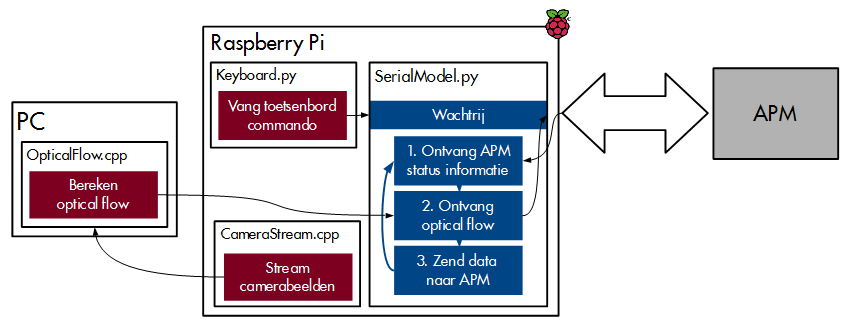
\includegraphics[width=0.9\linewidth]{RPIloop2}
	\caption{Schematische voorstelling van de nieuwe architectuur van het platform.}
	\label{fig:RPIloop2}
\end{figure}

\npar Het optical flow algoritme wordt uit de OpenCV bibliotheek ge\"importeerd \cite{url:opencv}. Zoals reeds eerder vermeld is optical flow tijdkritisch. Alle optical flow gerelateerde code wordt steeds in C ge\"implementeerd. C is dan ook de programmeertaal naar keuze bij tijdkritische applicaties \cite{paper:cpythonbenchmark}\cite{paper:cpythonbenchmark2}.

\subsubsection{CameraStream.cpp}
Aan de kant van RPi draait het programma $CameraStream.cpp$. Dit C programma wordt gebruikt om camerabeelden van de RPi naar de PC te versturen. CameraStream.cpp verstuurt de afmetingen van een frame naar de PC om vervolgens ieder nieuw frame onmiddellijk door te sturen. Alle data wordt verstuurd gebruik makend van een \textit{blocking send}. Zo wordt verzekerd dat CameraStream.cpp wacht om een nieuw frame te versturen wanneer het vorige nog niet volledig is ontvangen.

\subsubsection{OpticalFlow.cpp}
Aan de PC-kant draait $OpticalFlow.cpp$. Dit C programma staat in voor de berekening van optical flow. Via een \textit{blocking receive} worden eerst de afmetingen van ieder frame ontvangen. Ook via een \textit{blocking receive} wordt ieder nieuw frame ontvangen. De optical flow vectoren die hieruit resulteren worden dan met een \textit{non-blocking send} naar het serieel model op de RPi gestuurd. Op die manier kan OpticalFlow.cpp onmiddellijk het volgende frame ontvangen, zonder te moeten wachten tot het serieel model de flow vectoren heeft ontvangen.

\subsubsection{ZeroMQ}
Om communicatie tussen een C programma op de RPi en een C programma op de PC tot stand te brengen wordt gebruik gemaakt van de ZeroMQ bibliotheek \cite{url:ZeroMQ}. ZeroMQ werd gekozen omdat het een heel eenvoudige interface heeft. Bovendien is het ook makkelijk om berichten tussen Python en C programma's uit te wisselen. Deze eigenschap kan gebruikt worden om de berekende optical flow vectoren te sturen naar het serieel model op de RPi. Als communicatie protocol wordt TCP (Transmission Control Protocol) gekozen. TCP heeft een maximale pakketgrootte die kleiner is dan de grote van 1 frame. Om een camerabeeld van de RPi naar de PC te versturen moet het eerst worden onderverdeeld in een aantal deelpakketten. TCP is een \textit{best effort} protocol. Er wordt gebruik gemaakt van retransmissie indien pakketten verloren gaan. Het is belangrijk dat alle delen van een camerabeeld  worden ontvangen, anders kan het optical flow algoritme geen nuttige data opleveren.
% referentie naar ZeroMQ

\subsection{Compressie}
Het zou na\"ief zijn er vanuit te gaan dat het doorsturen van ruwe data van RPi naar PC de best mogelijke oplossing is. Compressie kan er in veel gevallen voor zorgen dat data sneller verstuurd wordt. Er moet gezocht worden naar een methode die weinig rekenkracht vergt aan de encoder kant, want die is nu eenmaal beperkt bij de RPi. Met deze voorwaarde in gedachten, wordt eerst gekozen voor LZ4. LZ4 behoort bij de beste compressie bibliotheken op vlak van encodeer- en decodeersnelheid \cite{url:quicklzbench}. Helaas is het niet gelukt om LZ4 werkend te krijgen op de RPi. Daarom wordt uiteindelijk gekozen voor QuickLZ \cite{url:quicklz}, ook \'e\'en van de betere compressie bibliotheken als het op snelheid aankomt \cite{url:quicklzbench}. QuickLZ werkt onmiddellijk zonder problemen.
% referentie naar quicklz vs others.
% referentie naar quicklz site

\subsection{Resultaat} \label{sec:resultaatVerleggen}
De snelheid van het optical flow algoritme wordt berekend aan de PC-kant door de tijd tussen twee opeenvolgende frames te meten. Dezelfde resoluties als in tabel \ref{table:resolutieTheorie} worden bekeken. Het gemiddeld aantal frames per seconde voor zowel met en zonder compressie wordt in tabel \ref{table:resolutieRPI} weergegeven.

% tabel met RPI1 no compr, compr FAST detector!!
\begin{table}
	\centering
	\caption{Het aantal frames per seconde gegeven de resolutie wanneer optical flow op de PC wordt berekend met Raspberry Pi 1 en Raspberry Pi 2}\label{table:resolutieRPI}
	\begin{tabular}{lcccc}
		\cr
		\hline
		& \multicolumn{2}{c}{Raspberry Pi 1} & \multicolumn{2}{c}{Raspberry Pi 2}\\
		\hline
		Resolutie & $FPS_{zonder\ compresie}$ & $FPS_{met\ compressie}$ & $FPS_{zonder\ compresie}$ & $FPS_{met\ compressie}$\\
		\hline
		160x120 & \SI{30.1}{\Hz} & \SI{29.9}{\Hz} & \SI{30.1}{\Hz} & \SI{30.1}{\Hz}\\
		320x240 & \SI{19.7}{\Hz} & \SI{15.5}{\Hz} & \SI{29.5}{\Hz} & \SI{29.7}{\Hz}\\
		640x480 & \SI{6.5}{\Hz} & \SI{5.1}{\Hz} & \SI{17.8}{\Hz} & \SI{12.6}{\Hz}\\
		\hline
	\end{tabular}
\end{table}

\npar In \ref{sec:quadcoptersturing} werd reeds aangehaald dat naar het einde van deze thesis toe, de RPi\,2 in gebruik genomen wordt. Het leek dan ook noodzakelijk om bovenstaande tests uit te voeren voeren voor de nieuwe versie van de RPi. De resultaten zijn ook opgelijst in tabel \ref{table:resolutieRPI}.

\npar Er kan besloten worden dat door het verleggen van het optical flow algoritme naar de PC, de resolutie verhoogd kan worden naar 320 bij 240 pixels om een zelfde frame rate te halen.  Voor de RPi\,1 wordt zonder compressie een frame rate van \SI{20}{\Hz} gehaald. De RPi\,2 haalt zelfs 30 frames per seconde, dit is de maximale snelheid waarmee de camera beelden kan registreren. Opmerkelijk is dat het gebruik van compressie niet zorgt voor betere prestaties. Zelfs een snelle compressie methode als QuickLZ blijkt te traag te werken op de RPi, waardoor compressie het aantal frames per seconde verlaagt in plaats van het te verhogen.

\npar Optical flow op de PC uitvoeren brengt wel \'e\'en groot nadeel met zich mee. Door de PC erin te betrekken wordt een extra vertraging toegevoegd. Dit wil zeggen dat de correcte optical flow data pas later beschikbaar zal zijn. Deze vertraging wordt gemeten in de APM en bedraagt drie tijdstappen en dus \'e\'en tijdstap meer dan voorheen. Waarschijnlijk zal dit geen probleem opleveren bij driftcompensatie.

\section{Optical Flow} \label{sec:OptFlowopt}
In de thesis van W. De Gucht werd een onderzoek gedaan naar de beste feature detector om optical flow mee te combineren. Good Features to Track (GFTT) \cite{paper:GFTT} bleek het best te presteren. De RPi is echter niet krachtig genoeg om deze detector te gebruiken voor een realtime toepassing. Daarom werd de Features from Accelerated Segment Test (FAST) \cite{paper:FAST} detector gebruikt. Gezien rekenkracht nu geen probleem meer mag zijn, wordt onderzocht of GFTT wel degelijk een betere prestatie oplevert. Eerst wordt de werking van beide detectors kort uitgelegd en vervolgens wordt hun prestatie vergeleken.

\subsection{FAST detector} \label{sec:FAST}
De FAST feature detector wordt beschreven door E. Rosten et al. in ``Machine learning for high-speed corner detection"\cite{paper:FAST}. Er wordt gebruik gemaakt van een getrainde decisieboom om te bepalen of een pixel een goeie feature is of niet.

\npar FAST heeft zijn naam niet gestolen. Deze detector werkt erg snel omdat geen zware berekeningen moeten gebeuren. Er moeten enkel een aantal geneste \textit{if-lussen} doorlopen worden.

\npar De detector heeft wel \'e\'en groot nadeel, FAST is erg gevoelig voor ruis. In de praktijk houdt dit in dat wanneer de quadcopter snel beweegt en de camerabeelden wazig worden, de detector veel minder goeie features vindt. Optical flow data is dan ook niet meer even betrouwbaar, wat belangrijke gevolgen kan hebben voor driftcompensatie.

\subsection{GFTT detector}
De GFTT feature detector wordt beschreven door J. Shi et al. in ``Good Features to Track"\cite{paper:GFTT}. Deze detector gaat features selecteren door ze te evalueren over meerdere frames. Er wordt een maat van ongelijkheid bijgehouden voor elke feature, die wordt ge\"updatet bij ieder nieuw frame. Wanneer een feature te veel begint te verschillen van hoe het er origineel uit zag, wordt de feature verwijderd uit de selectie. De resulterende feature verzameling is hierdoor optimaal voor het huidige frame. GFTT heeft wel als nadeel dat het veel meer rekenkracht eist dan de FAST detector.

\subsection{Resultaat}
Om de prestatie van beide detectors te vergelijken, wordt een zekere afstand afgelegd met de quadcopter in de hand. Er wordt afwisselend snel en traag gelopen, op die manier zullen zowel wazige als scherpe beelden geregistreerd worden. Alle camerabeelden worden opgeslagen en optical flow wordt berekend met beide detectors. De resulterende optical flow vectoren kunnen nu vergeleken worden om te zien welke detector het best presteert.

% figuur met scherpe beelden
\begin{figure}
\begin{center}

\subfigure[Frame 1]{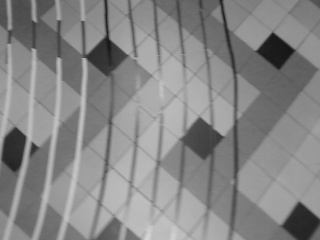
\includegraphics[width=0.45\linewidth]{TestScherp/frame1}}
\hspace{0.01\linewidth}
\subfigure[Frame 2]{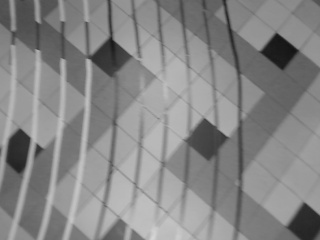
\includegraphics[width=0.45\linewidth]{TestScherp/frame2}}
\end{center}

\begin{center}
\subfigure[FAST]{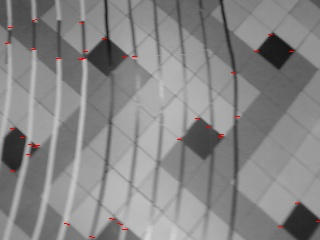
\includegraphics[width=0.45\linewidth]{TestScherp/FAST}}
\hspace{0.01\linewidth}
\subfigure[GFTT]{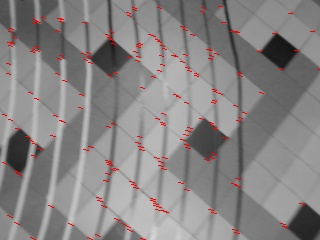
\includegraphics[width=0.45\linewidth]{TestScherp/GFTT}}
\end{center}
\centering
\caption{Flow vectoren voor optical flow in combinatie met FAST en GFTT voor scherpe beelden. Bij scherpe beelden vindt de GFTT detector(d) meer features dan de FAST detector(c). De features gevonden door beide detectors zijn van goeie kwaliteit.}\label{fig:scherp}
\end{figure}


\npar In figuur \ref{fig:scherp}(a) en \ref{fig:scherp}(b) zijn twee scherpe beelden te zien. De resulterende optical flow vectoren voor respectievelijk de FAST- en GFTT detector worden weergegeven in \ref{fig:scherp}(c) en \ref{fig:scherp}(d). Er kan afgeleid worden dat voor scherpe beelden, GFTT meer features vindt dan FAST.
% aanvullen met bevindingen

% figuur met wazige beelden
\begin{figure}
\begin{center}
\subfigure[Frame 1]{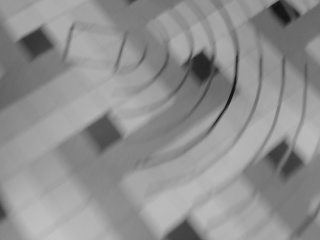
\includegraphics[width=0.45\linewidth]{TestWazig/frame1}}
\hspace{0.01\linewidth}
\subfigure[Frame 2]{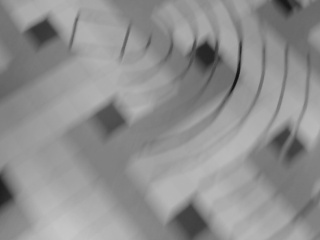
\includegraphics[width=0.45\linewidth]{TestWazig/frame2}}
\end{center}

\begin{center}
\subfigure[FAST]{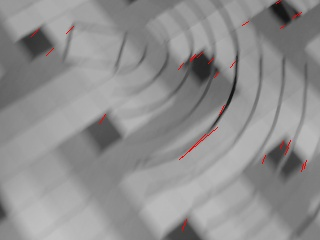
\includegraphics[width=0.45\linewidth]{TestWazig/FAST}}
\hspace{0.01\linewidth}
\subfigure[GFTT]{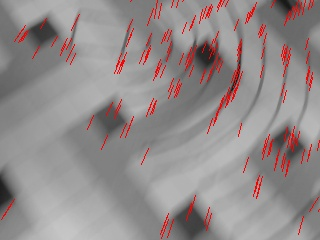
\includegraphics[width=0.45\linewidth]{TestWazig/GFTT}}
\end{center}
\centering
\caption{Flow vectoren voor optical flow in combinatie met FAST en GFTT voor wazige beelden. De GFTT detector(d) vindt duidelijk veel meer features dan de FAST detector(c) wanneer het beeld wazig wordt. Bovendien zijn de features die de FAST detector vindt niet allemaal van goeie kwaliteit, terwijl dit wel het geval is bij de GFTT detector.}\label{fig:wazig}
\end{figure}

\npar In figuur \ref{fig:wazig}(a) en \ref{fig:wazig}(b) zijn twee wazige beelden te zien. De beelden zijn wazig door de snelheid waarmee de quadcopter beweegt. De resulterende optical flow vectoren voor respectievelijk de FAST- en GFTT detector worden weergegeven in \ref{fig:wazig}(c) en \ref{fig:wazig}(d). GFTT bewijst zijn meerwaarde vooral bij wazige beelden. FAST vindt erg weinig flow vectoren, en enkele ervan zijn zijn zelfs niet correct. GFTT vindt een stuk meer flow vectoren die allemaal wel van degelijke kwaliteit zijn.

\npar Er kan geconcludeerd worden dat de GFTT detector een betere keuze is nu de rekenkracht geen probleem meer vormt. Deze detector zorgt ervoor dat de optical flow vectoren nog nauwkeuriger worden, ook wanneer het beeld wazig is.

\section{Hoogte regeling} \label{sec:hoogtereg}
In het werk van W. De Gucht werd de basis gelegd voor \textit{auto-takeoff} (automatisch opstijgen) en \textit{auto-land} (automatisch landen). Beide zijn nog voor verbetering vatbaar en worden in deze sectie besproken. Naast het opstijgen en landen moet de hoogteregeling tijdens het vliegen ook herzien worden. Het is heel erg belangrijk dat het platform mooi op dezelfde hoogte kan blijven vliegen omdat anders optical flow geen correcte resultaten kan geven. Voortdurend stijgen en dalen komt neer op continu in- en uitzoomen met de camera. Optical flow zal dan vectoren vinden in alle richtingen, wat absoluut niet wenselijk is. Daarom wordt de PID-regelaar geoptimaliseerd. Er wordt ook nagegaan of het gradueel verhogen van de gewenste hoogte naar een bepaalde setpoint minder overshoot oplevert.

\subsection{Auto-takeoff} \label{sec:autotakeoff}
Tijdens auto-takeoff, wordt gekeken naar de versnelling in de z-richting. Wanneer deze versnelling een zekere drempelwaarde overschrijdt, wordt \textit{lift-off} (het opstijgen zelf) gedetecteerd en gaat het platform over naar vliegmodus. Wanneer lift-off gedetecteerd wordt, slaat de APM de huidige throttlewaarde op  in de veronderstelling dat deze waarde ervoor zorgt dat het platform op \'e\'en bepaalde hoogte kan blijven vliegen. Deze throttlewaarde wordt vanaf nu ${Thr}_0$ genoemd.

\npar Deze aanpak is eigenlijk een manier om een ander probleem te omzeilen, het feit dat de batterij geen vast voltage levert naarmate ze leeg geraakt. Als de batterij een constante spanning zou leveren, dan zou ${Thr}_0$ altijd dezelfde waarde hebben. Helaas is er niet voldoende ruimte op het platform om hier nog een circuit voor te voorzien.

\npar De enige manier om een goede ${Thr}_0$ te vinden is dus door een optimale lift-off drempelwaarde in te stellen. Dit is uitermate belangrijk, want de correctie van de PID regelaars wordt rechtstreeks bij deze waarde opgeteld en terug naar de motoren gestuurd.

\npar Het vinden van de best mogelijke drempelwaarde is vrij eenvoudig. Er moet voor iedere drempelwaarde gekeken worden wat de gemiddelde correctie is die de hoogte regelaar moet uitvoeren om het platform op een constante hoogte te houden. De drempelwaarde, waarvoor de gemiddelde correctie het dichtst bij nul ligt, wordt behouden.

\subsection{Auto-land}
In de oorsponkelijke versie wordt de throttle te snel verminderd, waardoor de quadcopter een harde landing maakt. Dit wordt verholpen door de throttle waarde te verminderen naar een waarde net onder $Thr_0$. Op die manier gaat het platform gestaag dalen en kan een zachte landing gemaakt worden.

\subsection{Functiegenerator} \label{sec:functiegen}
De gebruikte sonar werkt aan \SI{20}{\Hz}. De hoogte regelaar wordt enkel opgeroepen wanneer nieuwe data van de sonar beschikbaar is. Wanneer een regelkring enkel op discrete tijdstippen kan worden bijgestuurd, wordt in de regeltechniek vaak de gewenste waarde gradueel opgevoerd naar de eigenlijke setpoint. De functie die de gewenste waarde moet beschrijven, wordt aangelegd met een zogenaamde \textit{functiegenerator}.

\npar Door het gebruik van een functiegenerator is het mogelijk om zowel snelheid en versnelling te beperken tot een maximum. Als versnelling en snelheid beperkt worden, dan wordt de kans op overshoot verkleind. 

\npar Stel, de maximale versnelling is $a_{max}$ en de maximale snelheid is $v_{max}$. In figuur \ref{fig:hsvprofiel} (a) is de functie te zien die aangelegd moet worden om van hoogte $h_1$ naar hoogte $h_2$ te gaan. De snelheid en versnelling worden ook geplot in respectievelijk (b) en (c).

\begin{figure}[htb]
\subfigure[Hoogte]{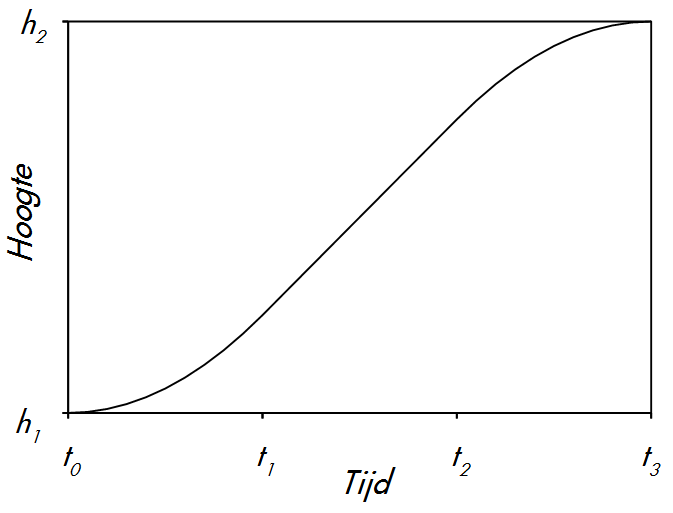
\includegraphics[width=0.31\linewidth]{HoogteRegeling/hoogte}}
\hspace{0.01\linewidth}
\subfigure[Snelheid]{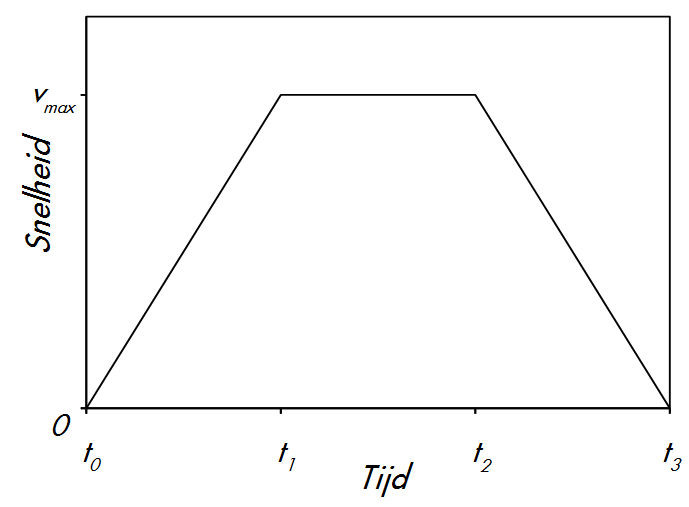
\includegraphics[width=0.31\linewidth]{HoogteRegeling/snelheid}}
\hspace{0.01\linewidth}
\subfigure[Versnelling]{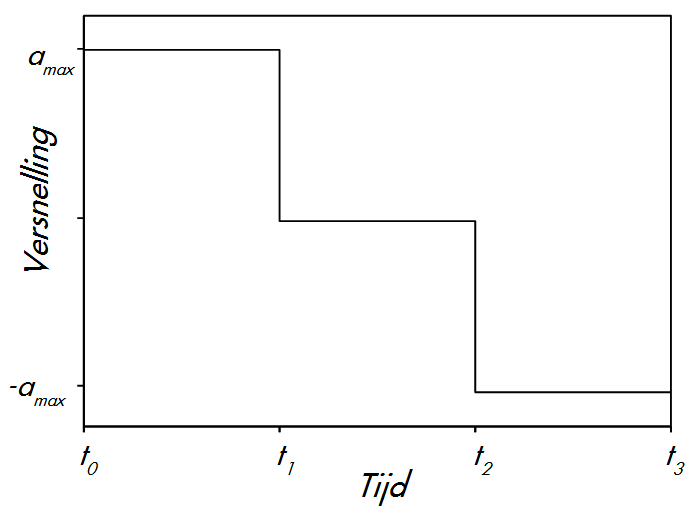
\includegraphics[width=0.31\linewidth]{HoogteRegeling/versnelling}}
\caption{Gewenst hoogte-, snelheids- en versnellingsprofiel}\label{fig:hsvprofiel}
\end{figure}

% referentie ERB
\noindent De profielen in figuur \ref{fig:hsvprofiel} kunnen voor iedere nieuwe setpoint berekend worden aan de hand van formules \eqref{eq:hoogtehoogtes} en \eqref{eq:hoogtetijden}. Deze formules zijn eenvoudig te vinden door de formules van de  \textit{\'e\'enparige rechtlijnige beweging} (ERB) om te vormen.

\begin{equation}
\left\{
\begin{matrix*}[l]

h(t) = h_1 + \frac{v_{max}^2}{2 \cdot a_{max}} \cdot t & \text{ als } t \leq t_1 \\
h(t) = h(t_1) + {v_{max}} \cdot t & \text{ als } t_1 < t \leq t_2 \\
h(t) = h(t_2) + \frac{v_{max}^2}{2 \cdot a_{max}} \cdot (t_2-t) & \text{ als } t_2 < t
\end{matrix*}
\right.
\label{eq:hoogtehoogtes}
\end{equation}

\begin{equation}
t_1 = \frac{v_{max}}{a_{max}},\ 
t_2 = (h_2-h_1)-\frac{v_{max}^{2}}{2 \cdot a_{max}}
\label{eq:hoogtetijden}
\end{equation}

\npar Bij implementatie van deze functiegenerator werd eerst een eenvoudigere versie geprogrammeerd. Deze eenvoudige versie beperkt enkel $v_{max}$. De gewenste hoogte neemt dan lineair toe met de tijd, tot de setpoint bereikt is. Uit de resultaten zal blijken dat deze eenvoudige aanpak ook volstaat.

\subsection{Optimalisatie PID parameters} \label{sec:optPID}
Na de optimalisaties in \ref{sec:autotakeoff} en \ref{sec:functiegen}, moet de hoogte regelaar ook eens bekeken worden. Om de ideale parameters te vinden, wordt gebruik gemaakt van de Ziegler-Nichols methode \cite{paper:ZieglerNichols}. De proportionele factor wordt opgedreven totdat de respons een oscillatie is met constante amplitude. De waarde voor de proportionele factor wordt de \textit{ultieme gain} genoemd. De ultieme gain wordt symbolisch voorgesteld als $K_u$. De oscillatieperiode wordt als $T_u$ voorgesteld. Volgens Ziegler-Nichols zijn de parameters die berekend kunnen worden met \eqref{eq:PIDpar} een goed uitgangspunt. 
\begin{equation}
	\centering
	P = 0.6 \cdot K_u,\ I = \dfrac{2 \cdot P}{T_u} \text{ en }D = \dfrac{K_p \cdot T_u}{8}
	\label{eq:PIDpar}
\end{equation}

\npar De met \eqref{eq:PIDpar} bekomen parameters zorgen nog voor zichtbare oscillaties. Bovendien is de responstijd vrij traag. De parameters moeten dus nog wat bijgeregeld worden. Om op een correcte manier te werk te gaan, wordt gesteund op het werk van K.\,H. Ang et al.\cite{paper:PIDtuning}. In deze paper wordt beschreven hoe een parameter moet aangepast worden om een bepaald effect te bekomen in het stapantwoord. Na een aantal tussenstappen wordt het gewenst gedrag bereikt. De proportionele- en differenti\"erende factor zijn nu wat hoger en de integrerende factor is verlaagd.

\subsection{Resultaat}
De optimalisatie van de drempelwaarde voor lift-off heeft vooral invloed op hoe snel het platform de gewenste hoogte bereikt net na het opstijgen. Als de lift-off waarde te laag gekozen wordt, dan is $Thr_0$ bijgevolg ook te laag. De integrerende factor moet dan de vaste fout op $Thr_0$ opvangen. Dit is te zien op figuur \ref{fig:opstijgen}(a). Wanneer de lift-off waarde wel goed gekozen wordt, zoals in figuur \ref{fig:opstijgen}(b), gaat het platform onmiddellijk naar de gewenste hoogte, weliswaar met een lichte overshoot.

\begin{figure}
	\begin{center}
		\subfigure[Lage lift-off drempelwaarde]{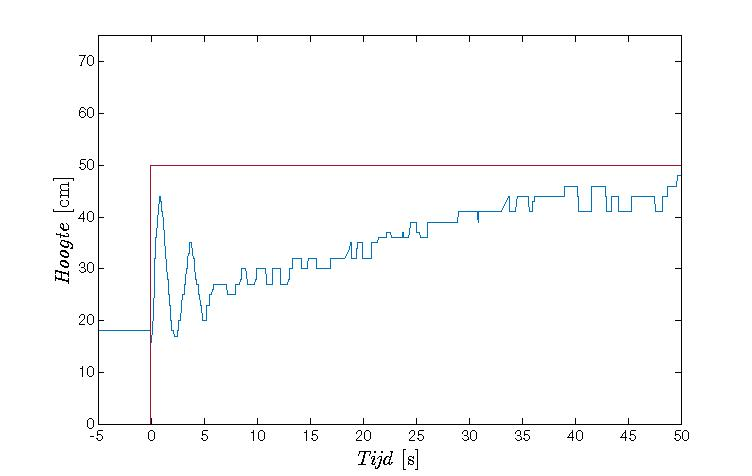
\includegraphics[width=0.8\linewidth]{HoogteRegeling/original}}
		
		\subfigure[Goede lift-off drempelwaarde]{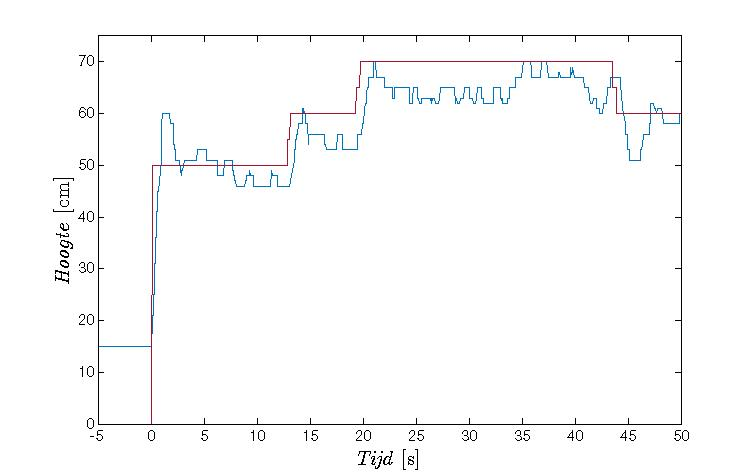
\includegraphics[width=0.8\linewidth]{HoogteRegeling/autotakeoff}}
	\end{center}
	\centering
	\caption{De invloed op het opstijggedrag van de quadcopter bij een te lage lift-off drempelwaarde in (a) en bij een goede lift-off drempelwaard in (b). Wanneer de drempelwaarde te laag gekozen is, duurt het een heel eind vooraleer de integrerende term van de PID-regelaar de vaste fout op $Thr_0$ heeft opgevangen.}\label{fig:opstijgen}
\end{figure}

\npar Overshoot is niet gewenst, dus die moet nog weggewerkt worden. Dit is de taak van de functiegenerator. Om de prestatie van de hoogte regeling zonder en met functiegenerator te vergelijken, wordt tijdens een testvlucht met de gewenste hoogte gespeeld. De reactie van het platform zonder en met functiegenerator wordt weergegeven in respectievelijk figuur \ref{fig:finaleHoogteRegeling}(a) en \ref{fig:finaleHoogteRegeling}(b). Het gebruik van een functiegenerator zorgt ervoor dat overshoot afneemt en dat de gewenste hoogte beter gevolgd wordt.

\begin{figure}
	\begin{center}
		\subfigure[Zonder functiegenerator]{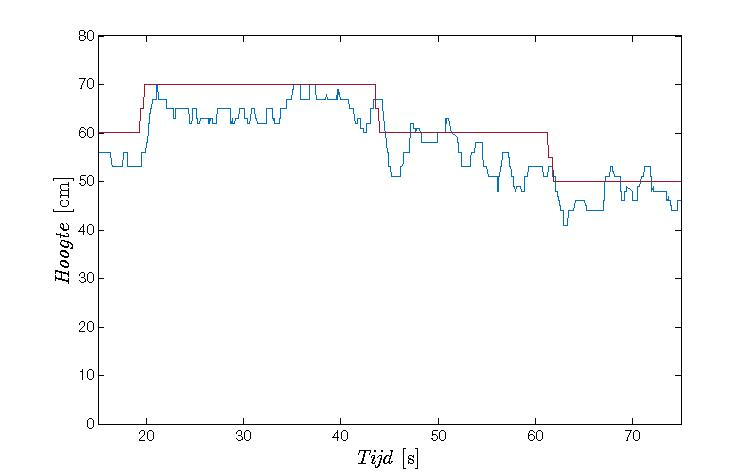
\includegraphics[width=0.8\linewidth]{HoogteRegeling/autotakeoffPID}}
		
		\subfigure[Met functiegenerator]{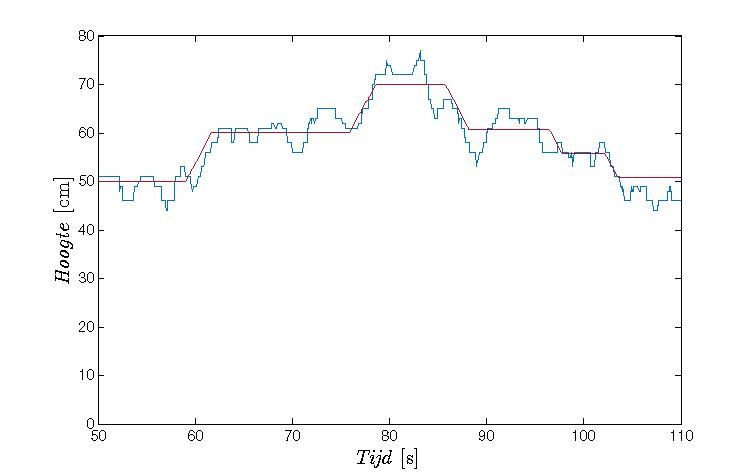
\includegraphics[width=0.8\linewidth]{HoogteRegeling/final}}
	\end{center}
	\centering
	\caption{Vergelijking tussen het vlieggedrag zonder en met functiegenerator. Wanneer de functiegenerator wordt aangezet, volgt de hoogte mooi de gewenste hoogte en is er minder overshoot dan wanneer de functiegenerator afligt.}\label{fig:finaleHoogteRegeling}
\end{figure}

\npar Er kan besloten worden dat het platform nu in staat is naar een bepaalde hoogte te navigeren zonder al te veel overshoot. De nieuwe hoogte regeling is in zijn opzet geslaagd. De optimalisatie van auto-land heeft weinig invloed op het vlieggedrag en wordt om die reden niet besproken bij de resultaten.


\section{Driftcompensatie}
In deze sectie wordt de driftcompensatie herzien. De drift van het platform wordt gemeten met behulp van optical flow. In \ref{sec:OptFlow} werd de werking van optical flow reeds uit de doeken gedaan. In sectie \ref{sec:OptFlowopt} werd de nauwkeurigheid van het algoritme verbeterd.

\npar Driftcompensatie op basis van optical flow is reeds aanwezig in de thesis van W. De Gucht, maar bij aanvang van deze thesis werkte dit helaas niet. Steunend op zijn werk wordt het opnieuw ingevoerd, met enkele aanpassingen weliswaar. Driftcompensatie kan gesplitst worden in twee delen. Op de eerste plaats moet de positie van het platform gemeten kunnen worden ten opzichte van de vorige positie. Pas dan kan drift gedetecteerd worden. Ten tweede is er de compensatie zelf. Van zodra drift gedetecteerd wordt, moet die gecompenseerd worden.

\subsection{Drift detecteren}
Het pijnpunt van de oorspronkelijke driftdetectie is dat er verondersteld wordt dat nieuwe optical flow data altijd met \SI{20}{\Hz} binnenkomt. Dit is in de praktijk echter niet het geval, er zit wat variatie op. Bijgevolg klopt de compensatie van de flow vectoren met roll en pitch niet volledig. Om dezelfde reden zijn de integratieterm en de differentiatieterm van de PID-regelaar ook niet correct. Door gewoon het tijdsverschil tussen de twee frames waarover optical flow berekend wordt mee te geven, kunnen deze twee problemen in \'e\'en keer worden opgelost.

\npar Er blijft echter wel nog steeds een probleem over bij de compensatie van de flow vectoren met roll en pitch. Door het verleggen van de optical flow berekeningen naar de PC, zit er een extra vertraging op de optical flow vectoren. Dit betekent dat de compensatie met roll en pitch verschoven moet worden. In \ref{sec:resultaatVerleggen} werd reeds vermeld dat de vertraging drie tijdstappen bedraagt.

\subsection{Drift compenseren}
Na het detecteren van drift moet er uiteraard ook compensatie volgen. Hiervoor moet de positie regelaar herzien worden. Deze wordt een stuk vereenvoudigd. Er wordt enkel nog gebruik gemaakt van een PI-regelaar die de snelheid regelt. De quadcopter kan dan in positie gehouden worden door zijn snelheid op nul te regelen.

\npar Om van positie te veranderen, wordt het wel iets ingewikkelder. Er moet gedurende een bepaalde tijd een gewenste snelheid opgelegd worden in de juiste richting. Deze snelheid moet dan weer naar nul gezet worden eens de positie bereikt is. In principe is dit volledig analoog aan hetgeen in \ref{sec:functiegen} werd toegepast. De positie zal lineair vari\"eren in functie van de tijd.

\subsection{Resultaten}
De nieuwe manier voor het compenseren van drift kan niet getest worden. Het platform reageert niet op de controlesignalen die worden aangelegd om pitch en roll te veranderen. Er wordt vermoed dat dit te wijten is aan het ontbreken van een afstandbediening. Normaal wordt de afstandbediening gebruikt voor het aanleggen van het gewenste vlieggedrag. Wanneer de afstandsbediening ontbreekt worden de variabelen die dit gedrag bijhouden niet correct ge\"initialiseerd. Bijgevolg is het niet mogelijk om het gewenst gedrag aan te passen.

\section{APM logica}
Naast het invoeren van optimalisaties moest ook heel wat code herschreven worden. Bij de code van W. De Gucht steunt de status van het platform voor een groot stuk op de signalen die gegeven worden door zijn afstandsbediening. Voor deze thesis was geen afstandbediening beschikbaar. Bovendien zijn een aantal statussen van het platform overbodig geworden, juist omdat er geen afstandsbediening meer gebruikt wordt. De nieuwe APM logica wordt afgebeeld in figuur \ref{fig:APMlogic}.

\begin{table}[h]
	\caption{Nieuwe commando's om het vlieggedrag te be\"invloeden.}\label{table:newcom}
	\centering
	\begin{tabular}{cp{.7\linewidth}}
		\cr
		\hline
		Commando & Betekenis \\
		\hline
		i & Auto-takeoff, de quadcopter laat zijn throttle stijgen tot lift-off wordt gedetecteerd. \\
		u & Auto-land, de quadcopter gaat langzaam dalen. \\
		y & Leg optical flow aan of uit.\\
		\hline	
	\end{tabular}
\end{table}


\npar De lijst met commando's die de RPi kan geven, is met drie commando's uitgebreid. Hun betekenis wordt nog eens opgelijst in tabel \ref{table:newcom}. Pas als optical flow wordt geactiveerd, kan een vaste positie aangehouden worden. Het is niet aangeraden om optical flow te activeren tijdens het opstijgen, zie \ref{sec:hoogtereg}.

\section{Besluit}
In dit hoofdstuk werden een aantal optimalisaties voorgesteld. Helaas werkt de driftcompensatie nog niet. Hoewel dit in theorie zou moeten werken is dit in praktijk niet het geval door het ontbreken van de afstandsbediening. Dit heeft belangrijke gevolgen voor de komende hoofdstukken over omgevingsmapping. De testen voor het mappen zullen steeds moeten gebeuren met de quadcopter in de hand.

\begin{figure}[h]
	\centering
	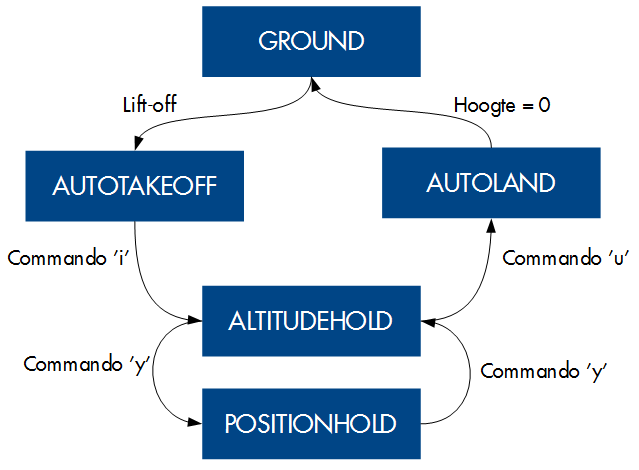
\includegraphics[width=0.7\linewidth]{APMlogic}
	\caption{Logica op de APM. De statussen worden afgebeeld in de rechthoeken. De condities voor een transitie worden afgebeeld naast de pijlen.} \label{fig:APMlogic}
\end{figure}




% !TeX spellcheck = nl_NL
\chapter{SLAM}\label{sec:SLAM}
In de inleiding van deze thesis werd reeds vermeld dat voor het mappen van de omgeving van de quadcopter beroep zou gedaan worden op \textit{Simultaneous Localisation and Mapping} (SLAM). In dit hoofdstuk worden de algoritmes in reeds bestaande werken bekeken en wordt de keuze van het SLAM algoritme in deze thesis toegelicht.

\section{Laserscanner}
De keuze voor een laserscanner ligt reeds vast sinds de probleemstelling. Toch wordt even de tijd genomen om hier verder op in te gaan. Het grote voordeel van een laserscanner is gekend, diepte informatie kan er rechtstreeks worden uitgehaald. Bij een camera is dit niet zo, maar kan er wel heel veel andere informatie uitgehaald worden.

\npar Het blijft de bedoeling om het platform volledig autonoom te houden. Als optical flow online moet gebeuren, wordt reeds heel wat rekenkracht gebruikt voor driftcompensatie. Om zeker niet in de problemen te komen, is het dus beter geen visueel SLAM algoritme te gebruiken. Een laserscanner is dus beter geschikt voor het platform.

% Het is wel belangrijk om op te merken dat er enkel horizontaal gemeten wordt. Als het platform lichtjes kantelt, dan wijst de laserscanner de verkeerde kant uit. Dit fenomeen is weergegeven in figuur xxx [ref]. Het zal dat nodig zijn om de meting van de laserscanner te compenseren met de gemeten roll en pitch van de quadcopter.

\section{Twee paradigmas}
Wanneer men SLAM implementeert, moet gekozen worden voor een algoritme dat ofwel \textit{Extended Kalman filters} (EKF) ofwel \textit{Particle filters} gebruikt. De voor- en nadelen worden hieronder besproken. De basis voor beide paradigma's blijft echter wel gelijk. Daarom wordt dit eerst uitgelegd. Het basisalgoritme is ook weergegeven in figuur \ref{fig:SLAMprin}.

% figuur SLAM
\begin{figure}
	\centering
	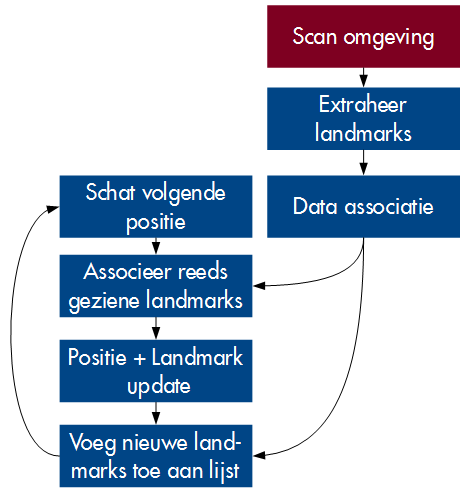
\includegraphics[width=0.5\linewidth]{SLAMprinciple}
	\caption{Grafische voorstelling van het basisalgoritme voor SLAM.} \label{fig:SLAMprin}
\end{figure}

\npar Bij iedere SLAM implementatie wordt een lijst aangelegd met zogenaamde \textit{landmarks}. Dit zijn referentiepunten, die in het geval van omgevingsmapping overeen stemmen met ofwel muurpunten ofwel obstakels in de ruimte die in kaart moet worden gebracht. Een quadcopter kan gebruik maken van de afstand tot de verschillende landmarks om zijn eigen positie te berekenen. Als nieuwe data beschikbaar is, worden hier eerst landmarks uit ge\"extraheerd. Op basis van de geschatte positie van het platform worden de ge\"extraheerde landmarks vergeleken met de reeds geziene landmarks. Deze vergelijking stelt het algoritme in staat de schatting te corrigeren door de positie van het platform en de landmarks te updaten. Eens de nieuwe positie gekend is, kan de locatie van de niet eerder geziene landmarks ook bepaald worden. Als het platform over odometrie beschikt, dan wordt dit vaak gebruikt om het schatten van de volgende positie nauwkeuriger te maken.

\npar De hierboven aangehaalde paradigma's verschillen in de manier waarop de nieuwe positie van de quadcopter en de positie van de landmarks wordt geschat.

\npar Voor de volledigheid wordt een derde paradigma vermeld. Graaf-gebaseerde optimalisatie technieken. Dit paradigma wordt in de praktijk zelden gebruikt voor online toepassingen en wordt daarom ook niet verder besproken \cite{book:SLAMHandbook}.

\subsection{Extended Kalman Filters}
De positie van de quadcopter en de positie van alle landmarks zijn allemaal stochastische variabelen. Er wordt verondersteld dat ze gemeenschappelijk gaussiaans verdeeld zijn. Een gaussiaanse verdeling met meerdere variabelen wordt getypeerd door een schatting van iedere variabele, de verwachtingswaarde en een schatting op de fout van die verwachtingswaarde, de covariantiematrix. Als een nieuwe scan beschikbaar is en er worden reeds geziene landmarks waargenomen, dan worden alle verwachtingswaarden en de volledige covariantiematrix ge\"updatet. Als er nieuwe landmarks worden gezien, dan worden die toegevoegd als extra variable aan de gaussiaanse verdeling. Het updaten van de verwachtingswaarden en de covariantiematrix, of anders verwoord het schatten van de nieuwe verwachtingswaarden en de covariantiematrix gebeurt aan de hand van Extended Kalman filters \cite{book:SLAMHandbook}.

\npar Het is zo dat EKF-SLAM na verloop van tijd altijd inconsistent wordt. Dit door het feit dat uitgegaan wordt van een gaussiaanse verdeling, terwijl de feitelijke verdeling voor de robotpositie en landmarks iets helemaal anders kan zijn \cite{paper:SLAMconsistency}.

\npar Om telkens opnieuw deze volledige covariantiematrix te updaten is veel rekenkracht nodig. Bovendien moeten ook voortdurend nieuwe landmarks worden toegevoegd wanneer nieuw terrein wordt verkend. Dit zorgt ervoor dat er nog meer berekeningen moeten gebeuren. Als antwoord op dit nadeel werd FastSLAM ontwikkeld \cite{paper:FastSLAM}. Dit is \'e\'en van de eerste SLAM algoritmes die gebruik maakt van particle filters \cite{paper:SLAMTutorial}.

\subsection{Particle Filters}
Het gebruik van particle filters voor het in kaart brengen van een onbekende omgeving werd ge\"introduceerd door K.P. Murphy \cite{paper:BayesianMap}. De eerste toepassing van zijn idee\"en volgde pas enkele jaren later met FastSLAM \cite{paper:FastSLAM}. De map en de positie van de quadcopter worden van elkaar losgekoppeld. Er worden meerdere partikels bijgehouden. Dit zijn als het ware mogelijke staten waarin het platform zich kan bevinden. Voor ieder partikel wordt een map bijgehouden. De punten worden opnieuw als guassiaans verdeeld ondersteld. Doordat de positie werd losgekoppeld van de map, zijn de landmarks niet langer afhankelijk van elkaar. Dit betekent dat ieder punt van een 2D map kan voorgesteld worden door een 2D verwachtingswaarde en een 2x2 covariantiematrix. Wanneer een nieuwe scan toekomt, wordt eerst de nieuwe positie geschat voor ieder partikel. Vervolgens wordt aan de hand van die schatting, voor ieder partikel de bijhorende verwachtingswaarde en covariantiematrix van alle landmarks ge\"updatet met een Kalman filter.

\npar Waar EKF-SLAM een gigantische matrix moest updaten, moet bij het gebruik van een particle filter, voor ieder partikel, voor iedere landmark de verwachtingswaarde en de covariantie matrix worden ge\"updatet. De complexiteit van de berekeningen bij een particle filter zullen dus lineair stijgen met het aantal landmarks. Bij EKF-SLAM stijgt de complexiteit kwadratisch. In FastSLAM worden landmarks dan nog eens georganiseerd in een boomstructuur. Dit zorgt ervoor dat complexiteit van de berekeningen logaritmisch schaalt met het aantal landmarks. Er kan besloten worden dat het gebruik van een particle filter een stuk minder zware berekeningen vergt \cite{paper:FastSLAM} \cite{book:SLAMHandbook}.

\subsection{Besluit}
Uit een korte literatuurstudie is gebleken dat er best geopteerd wordt voor een SLAM algoritme dat gebruik maakt van particle filters. Het is de bedoeling dat de map realtime gegenereerd wordt, dus de nodige rekenkracht moet beperkt blijven. Zeker omdat het uiteindelijk de bedoeling is het SLAM algoritme online op de quadcopter te laten draaien zodat het platform zelf kan beslissen naar waar gevlogen wordt om een volledige ruimte of misschien zelfs een volledig gebouw te verkennen. Hetzelfde besluit wordt gemaakt in werken gelijkaardig aan deze thesis \cite{paper:sameasme1} \cite{paper:sameasme2}.

\section{BreezySLAM}
Gezien de beperkte rekenkracht van het gebruikte platform is een algoritme dat gebruik maakt van particle filters aangewezen. Er zijn heel veel open source SLAM implementaties beschikbaar. Er wordt gezocht naar een implementatie die eenvoudig te verzoenen is met de architectuur van het platform in deze thesis. Bovendien wordt eerst gekeken naar SLAM implementaties die 2D mappen genereren. Pas wanneer het platform in staat is een goeie 2D map te maken, kan er gekeken worden of 3D mappen ook haalbaar zijn met de aanwezige hardware.

\npar \textit{HectorSLAM} wordt reeds gebruikt voor omgevingsmapping met een quadcopter in het werk van M. G\"abel et al. \cite{paper:sameasme1}\cite{paper:hectorSLAM}. Deze implementatie heeft als belangrijk voordeel dat er rekening wordt gehouden met de roll en pitch van het platform. Waarom dit belangrijk is wordt ge\"illustreerd in figuur \ref{fig:lasercomp}. Wanneer een quadcopter lichtjes kantelt, zijn de metingen van de laserscanner niet meer volledig correct. HectorSLAM is beschikbaar in het ROS raamwerk \cite{url:hectorROS}. Om HectorSLAM werkende te krijgen op de PC wordt op vrij veel problemen gestoten. Daarom wordt verder gezocht naar een andere implementatie.

\begin{figure}[h]
	\centering
	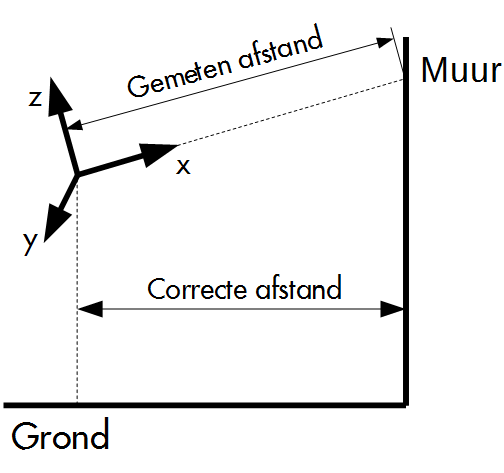
\includegraphics[width=0.40\linewidth]{lasercomp}
	\caption{Het assenstelsel op de figuur geeft de houding van een quadcopter weer. Er wordt ge\"illustreerd waarom de gemeten afstanden niet volledig kloppen wanneer het platform kantelt in een bepaalde richting.} \label{fig:lasercomp}
\end{figure}

\npar Wat wel makkelijk te integreren zou zijn is een implementatie die geschreven is in C of in Python, gezien deze twee talen reeds gebruikt werden voor het platform. Een zeer lichte C implementatie voor SLAM is \textit{TinySLAM} \cite{paper:tinySLAM} \cite{paper:tinySLAM2}. Zoals de naam al doet vermoeden, bestaat TinySLAM uit minder dan 200 lijnen code. Uit figuur \ref{fig:tinyslammap} blijkt het degelijk te presteren. Uiteindelijk wordt gekozen voor \textit{BreezySLAM} \cite{thesis:BreezySLAM} \cite{url:BreezySLAMlib}, een implementatie afgeleid van TinySLAM, omdat het een stuk gebruiksvriendelijker is. TinySLAM en BreezySLAM laten beide het gebruik van odometrie toe, maar roll en pitch horen daar niet bij. Er moeten dus maatregelen genomen worden om de roll en pitch te compenseren in de laserdata.

\begin{figure}[h]
	\centering
	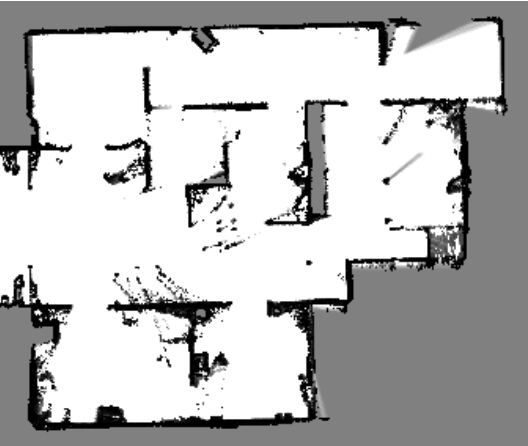
\includegraphics[width=0.31\linewidth]{tinySLAMmap}
	\caption{2D map gegenereerd met TinySLAM.} \label{fig:tinyslammap}
\end{figure}

% !TeX spellcheck = nl_NL
\chapter{Integratie SLAM in het platform}
In dit hoofdstuk wordt het gekozen SLAM algoritme ge\"integreerd in het huidige platform. Er moeten eerst een aantal aanpassingen gemaakt worden aan de architectuur, zowel op vlak van hardware als op vlak van software. Eens de architectuur af is, wordt de prestatie van het SLAM algoritme ge\"evalueerd. Dit gebeurt eerst zonder odometrie van de quadcopter te gebruiken, om erna te zien wat het effect is als er wel odometrie gebruikt wordt. In dit hoofdstuk moet in het achterhoofd gehouden worden dat het uiteindelijke doel erin bestaat dat de quadcopter autonoom een omgeving kan verkennen. Er moet dus ook nagegaan worden of dit mogelijk is met het gebruikte platform.

\section{Aanpassingen architectuur}

\subsection{Aanpassingen hardware}
Om aan SLAM te doen, wordt in dit werk een URG-04LX-UG01 laserscanner van Hokuyo gebruikt. Deze laserscanner haalt een maximale scanfrequentie van \SI{10}{\Hz}. Deze scanner kan gewoon via USB aangesloten worden. Dit levert echter een probleem op, want de RPi\,1 heeft slechts 2 USB-poorten en die zijn reeds in gebruik door de WiFi-dongle en de camera. Omdat het niet mogelijk is nog een USB-HUB toe te voegen aan het platform wegens plaatsgebrek, moet een andere optie gezocht worden. De beste oplossing lijkt ons over te gaan naar de nieuwe RPi\,2. Deze is een stuk krachtiger, en beschikt over 4 USB-poorten, zie tabel \ref{table:RP1vsRPI2}.

\npar Van de gebruikte laserscanner is geweten dat hij vrij veel stroom eist. Dit blijkt dan ook meteen een probleem op te leveren. De RPi2 kan niet voldoende stroom  leveren om zowel de laserscanner als de camera voldoende te voeden. De RPi2 wordt gevoed door de APM. Als de laserscanner ook rechtstreeks gevoed wordt door de APM lijkt dit probleem reeds opgelost. Een foto van de finale versie van het platform is weergegeven in figuur \ref{fig:quadfinal}.

\begin{figure}[h]
	\centering
	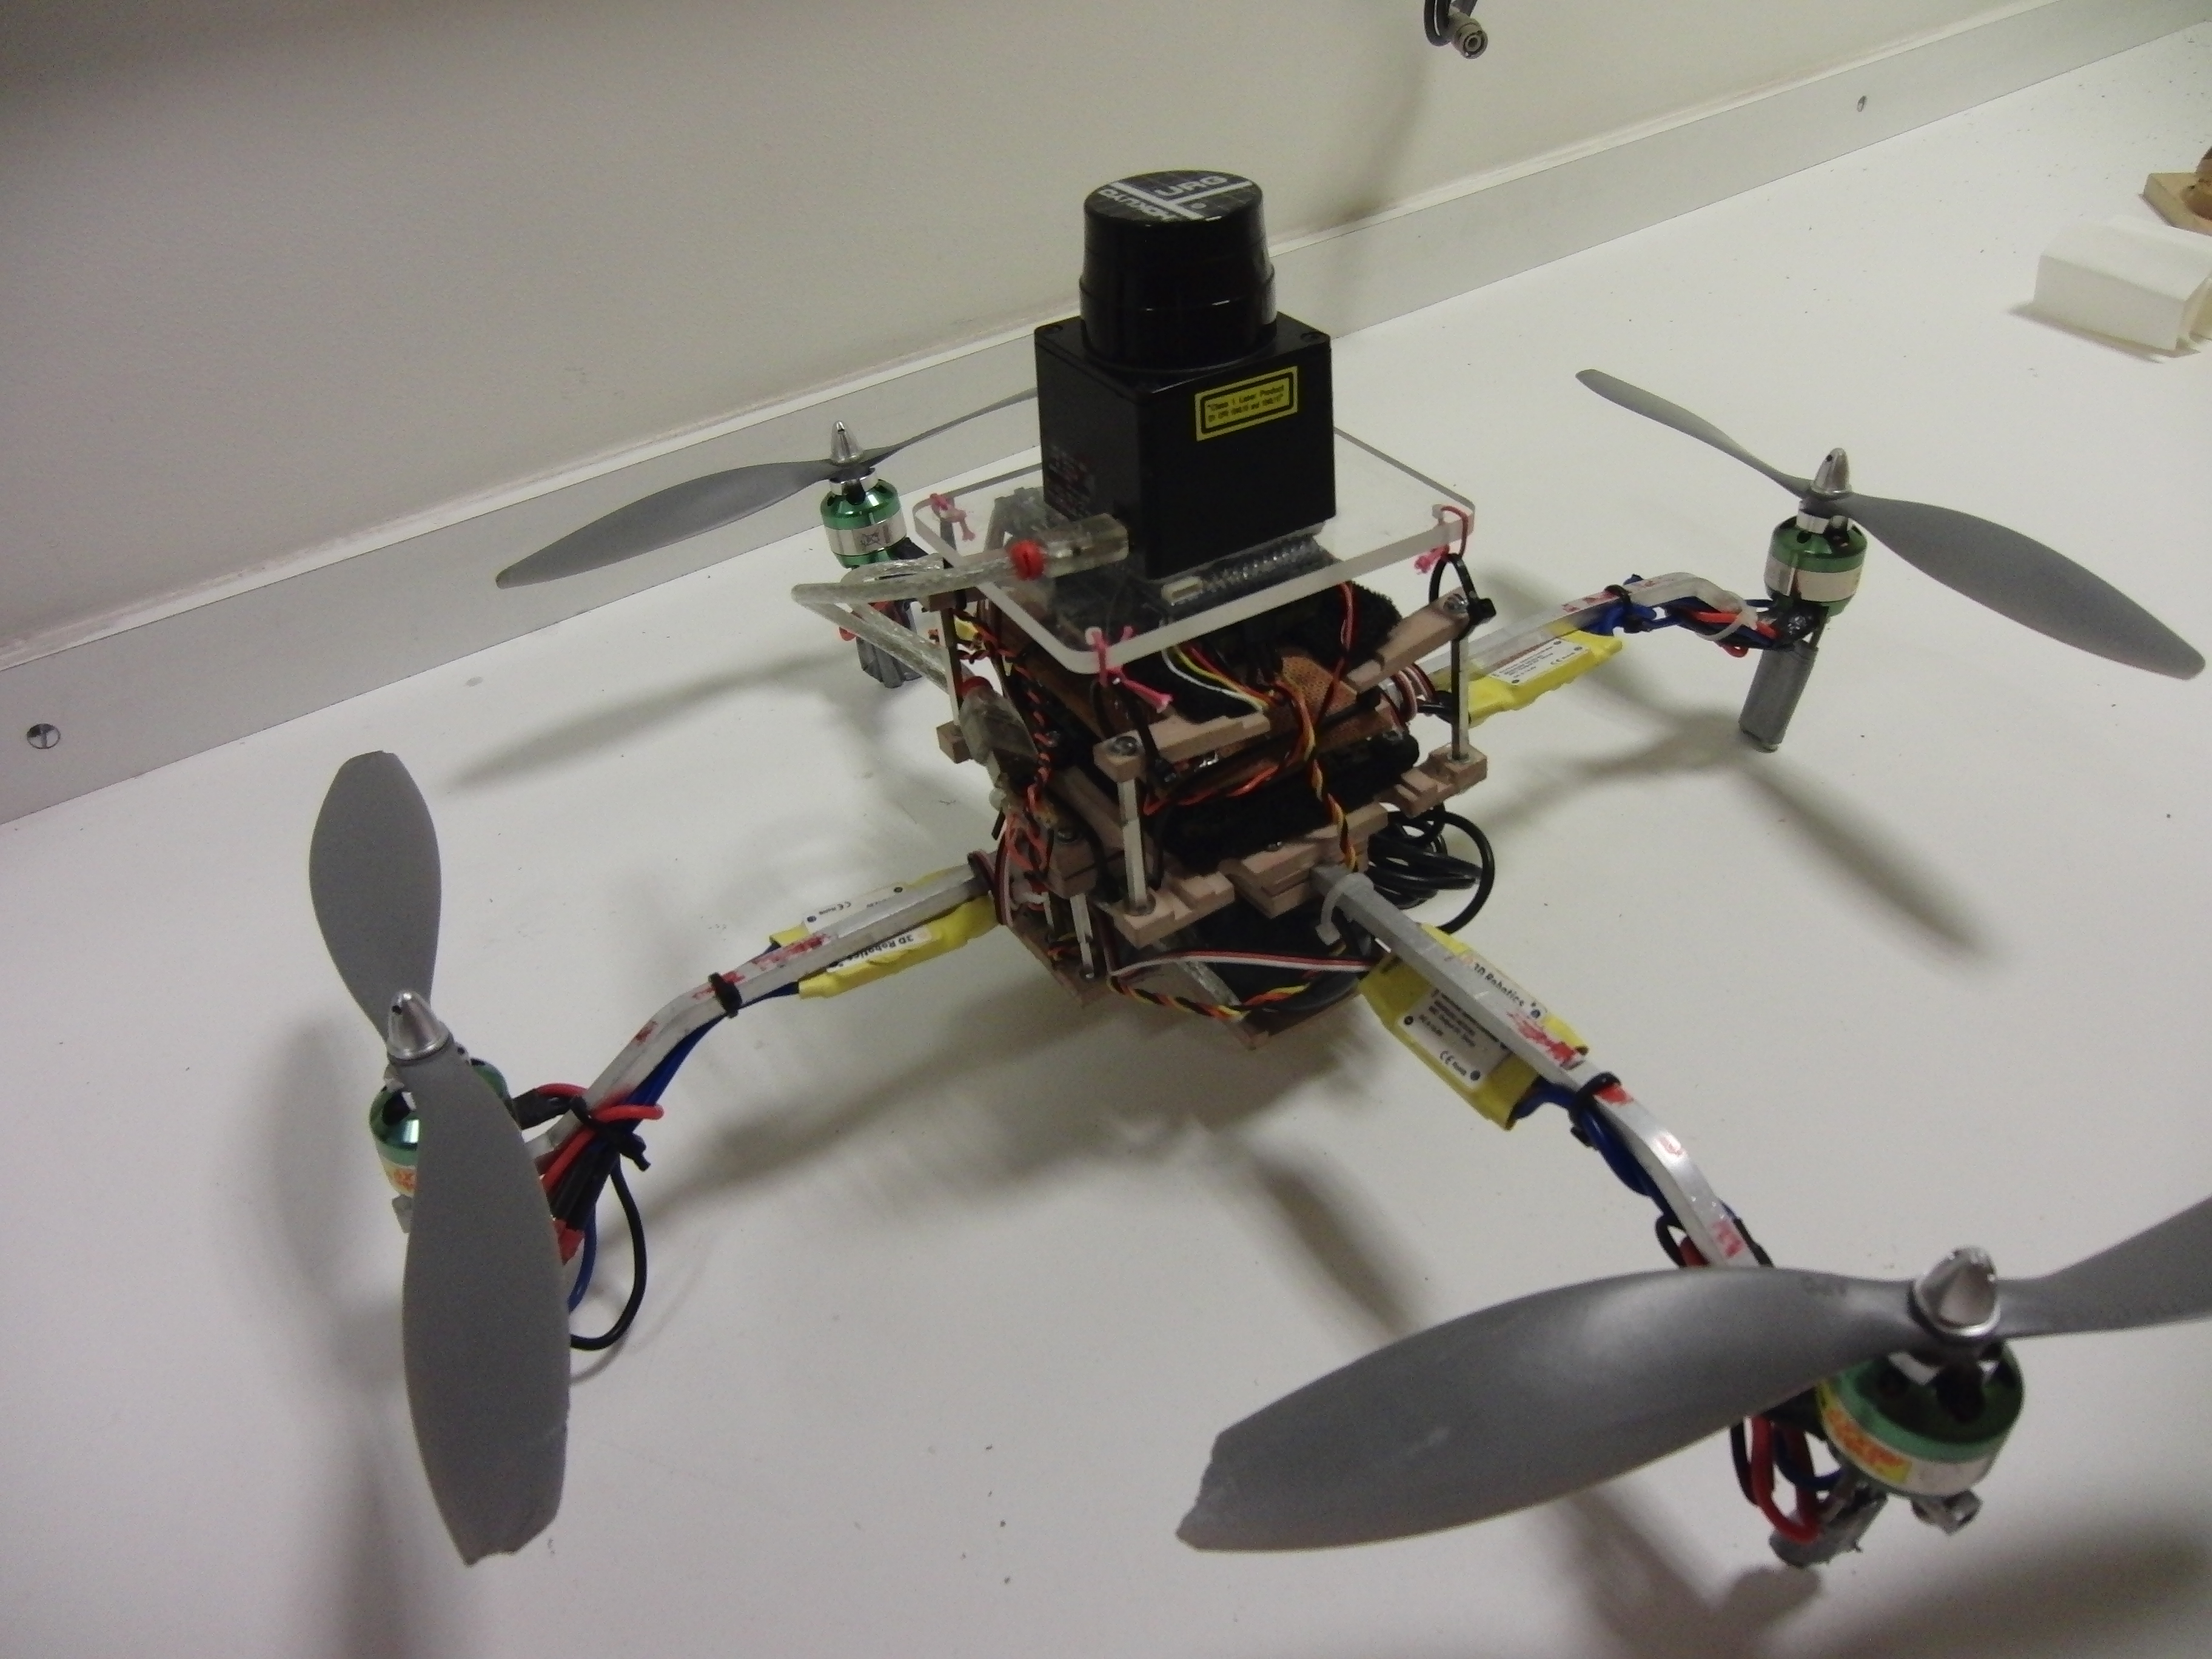
\includegraphics[width=0.65\linewidth]{quadfinal}
	\caption{Het platform wordt in deze figuur weergegeven. De laserscanner is gemonteerd bovenaan de het frame.}\label{fig:quadfinal}
\end{figure}

\subsection{Aanpassingen software}
De nieuwe softwarearchitectuur wordt afgebeeld in figuur \ref{fig:RPIloop3a}. Er verandert echter niets aan de software op de APM, daarom wordt deze niet in detail weergegeven. In de figuur is te zien dat de PC nu twee programma's moet draaien: \textit{SLAM.cpp} en \textit{OpticalFlow.cpp}. Aan de Raspberry Pi kant komt er ook een programma bij: \textit{LaserStream.cpp}.

\begin{figure}[h]
	\centering
	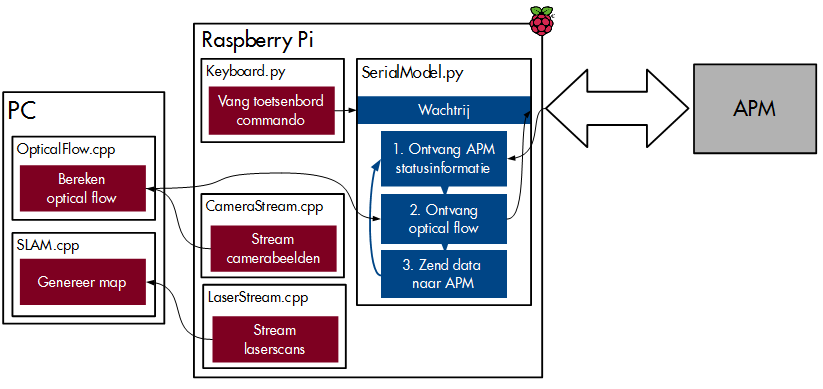
\includegraphics[width=0.8\linewidth]{RPIloop3a}
	\caption{Nieuwe softwarearchitectuur van het platform.}\label{fig:RPIloop3a}
\end{figure}

\subsubsection{LaserStream.cpp}
De naam van dit programma spreekt voor zich. Het is een C programma dat voortdurend scans van de laserscanner doorstuurt naar SLAM.cpp. Voor het versturen wordt een \textit{blocking send} gebruikt. De volgende scan kan pas verstuurd worden wanneer de vorige is ontvangen. Voor het versturen van de scans kunnen de communicatieklassen gebruikt worden die geschreven werden voor de optical flow berekening.

\subsubsection{SLAM.cpp}
SLAM.cpp moet de map genereren met als input de laserscans. Deze worden ontvangen met een \textit{blocking receive}. Het is dan ook niet meer dan logisch dat de volgende schatting van de map pas gemaakt wordt wanneer de nieuwe scan volledig is ontvangen. BreezySLAM voorziet een C bibliotheek met een eenvoudige interface. Deze bibliotheek wordt dan ook gebruikt om het SLAM algoritme te implementeren.

\section{SLAM zonder odometrie}
Eerst wordt het SLAM algoritme ge\"evalueerd zonder het gebruik van odometrie. Het algortime blijkt reeds goed te presteren in een kleine ruimte, zolang \'e\'en bepaalde plaats geen twee maal bezocht wordt. Dit wordt in de literatuur het \textit{loop-closing} probleem genoemd \cite{book:SLAMHandbook}. Als een bepaalde plaats niet herkend wordt wanneer ze voor de twee keer wordt bezocht, dan begint het SLAM algoritme fouten te maken. Een voorbeeld van een kleine map is te zien in figuur \ref{fig:loopclosing}(a). Wanneer een extra rondje gedaan wordt in dezelfde kamer ziet de map eruit als in figuur \ref{fig:loopclosing}(b). Er kan duidelijk gezien worden dat de kamer twee keer boven elkaar wordt getekend. De twee tekeningen van de kamer zijn wat geroteerd ten opzichte van elkaar. Dit doet vermoeden dat het gebruik van odometrie en in het bijzonder, het toevoegen van de yaw van de quadcopter, de gegenereerde map kan verbeteren.

%figuur A kamer 1 rond, B kamer 2 rond
\begin{figure}[h]
	\centering
	\subfigure[Map gegenereerd na \'e\'en rondje in een kamer.]{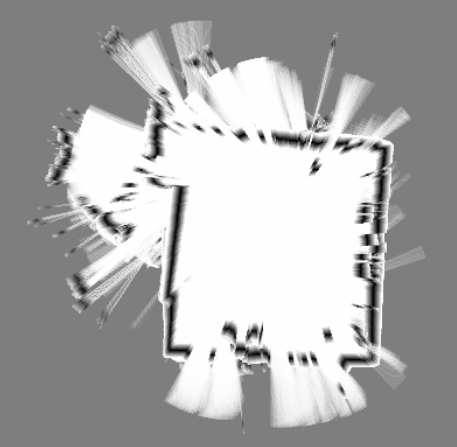
\includegraphics[width=0.40\linewidth, height=6cm]{SLAM/noodo1ROOM}}
	\hspace{0.01\linewidth}
	\subfigure[Map gegenereerd na twee rondjes in een kamer.]{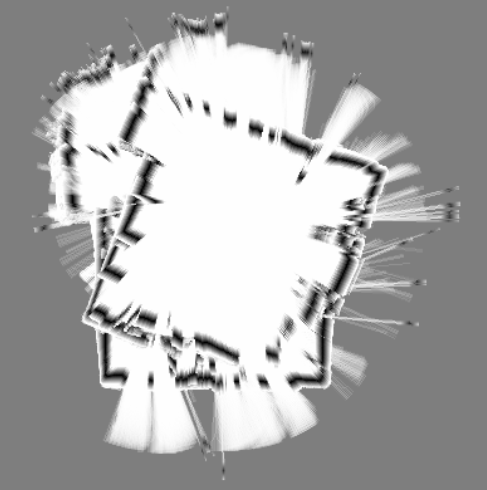
\includegraphics[width=0.40\linewidth, height=6cm]{SLAM/loopclosure}}
	\caption{Het loop-closing probleem: de invloed van eenzelfde plaats twee keer bezoeken. BreezySLAM herkent de plaatsen niet wanneer deze de tweede keer worden bezocht. Hierdoor wordt een nieuwe map getekend bovenop de map die er reeds getekend was.} \label{fig:loopclosing}
\end{figure}

\section{SLAM met odometrie}
Voor het toevoegen van odometrie moeten eerst weer een aantal aanpassingen komen aan de software architectuur. Deze worden eerst beschreven om vervolgens over te gaan tot de resultaten. De finale versie van de architectuur is afgebeeld in figuur \ref{fig:RPIloop3}.

\begin{figure}[h]
	\centering
	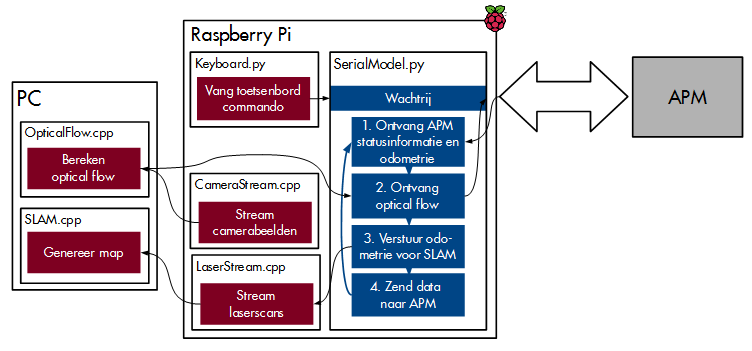
\includegraphics[width=0.8\linewidth]{RPIloop3}
	\caption{De aangepaste architectuur, die SLAM voorziet van odometrie.} \label{fig:RPIloop3}
\end{figure}

\subsection{Aanpassingen softwarearchitectuur}
De odometrie moet vanop de APM tot aan SLAM.cpp op de PC geraken. BreezySLAM vraagt de voorwaartse verplaatsing, het verschil in yaw en het tijdsverschil waarover deze twee werden gemeten als odometrie. Het aanpassen van de APM is triviaal gezien dit gewoon betekent dat specifieke statusinformatie geprint moet worden naar de RPi. Binnen SLAM.cpp moet de odometrie gewoon als extra parameter meegegeven worden aan BreezySLAM. De andere aanpassingen zijn iets minder triviaal en worden daarom wat uitgebreider beschreven. Het compenseren van de laserscans met roll en pitch van het platform wordt voorlopig nog niet ge\"implementeerd omdat er verondersteld wordt dat de quadcopter gedurende zijn vlucht altijd ongeveer evenwijdig met de grond blijft vliegen.

\subsubsection{SerialModel.py}
In het serieel model, \textit{SerialModel.py}, van de RPi moet de statusinformatie met odometrie doorgewezen worden naar het programma LaserStream.cpp. De software van de RPi zal er uit zien zoals op figuur \ref{fig:RPIloop3}. Er is een taak bijgekomen in de lus. Telkens wanneer odometrie beschikbaar is wordt die met een \textit{blocking send} doorgestuurd naar het programma LaserStream.cpp.

\subsubsection{LaserStream.cpp}
In LaserStream.cpp wordt een aparte thread aangemaakt die voortdurend wacht tot er nieuwe odometrie beschikbaar is. Om de odometrie te ontvangen wordt een \textit{blocking receive} gebruikt. Odometrie wordt ge\"updatet aan de snelheid waarmee een nieuwe voorwaartse verplaatsing beschikbaar is. Uit tabel \ref{table:resolutieRPI} bleek dat dit voor de RPi2 aan \SI{30}{\Hz} is. Om het verschil in snelheid tussen de odometrie en de laserscan op te vangen, wordt de odometrie geaggregeerd zolang er geen scan beschikbaar is. Wanneer een nieuwe scan klaar is om te verzenden wordt de geaggregeerde odometrie eraan toegevoegd. Om ervoor te zorgen dat dit alles \textit{thread-safe} gebeurt, wordt gebruik gemaakt van een \textit{mutex}.

\subsection{Resultaat}
Om het resultaat van de toevoeging van de odometrie te kunnen evalueren wordt telkens vergeleken met de resultaten zonder odometrie. In figuur \ref{fig:BreezyRes}(a) en \ref{fig:BreezyRes}(b) wordt een map weergegeven van \'e\'en kamer respectievelijk zonder en met odometrie. In figuur \ref{fig:BreezyRes}(c) en \ref{fig:BreezyRes}(d) wordt een map weergegeven van drie kamers respectievelijk zonder en met odometrie.

\npar Voor het mappen van \'e\'en kamer is de prestatie met en zonder odometrie ongeveer dezelfde. Wanneer meerdere kamers in kaart worden gebracht, draaien ze wat ten opzichte van elkaar als geen odometrie wordt gebruikt. Wanneer wel rekening gehouden wordt met odometrie, liggen de kamers correcter naast elkaar.

\npar In figuur \ref{fig:loopclosing2} wordt het loop-closing probleem zonder en met odometrie vergeleken. Ook met odometrie heeft BreezySLAM het moeilijk om een goede map te genereren wanneer een bepaalde plaats meer dan eens wordt bezocht. Het ontbreken van een loop-closing strategie blijft een pijnpunt. Het huidige algoritme moet dus uitgebreid worden om betere mappen te kunnen genereren. Overstappen naar een ander algoritme, dat wel aan loop-closing doet is ook een optie.

\npar Om te zien of het op termijn mogelijk zou zijn om de RPi\,2 te gebruiken voor omgevingsmapping zonder hulp van de PC, wordt al eens gekeken naar het CPU gebruik bij het uitvoeren van BreezySLAM. Dit blijkt 37\% te bedragen. Een zwaarder algoritme draaien is dus nog mogelijk.

\section{Besluit}
Het toevoegen van odometrie aan BreezySLAM zorgt reeds voor betere mappen. Toch zijn ze nog niet nauwkeurig genoeg. De reden voor deze ondermaatse prestatie ligt bij het ontbreken van een loop-closing stategie. TinySLAM doet wel aan loop-closing en is dus een optie. HectorSLAM doet niet aan loop-closing, maar uit onderzoek blijkt dat het algoritme toch nauwkeurig genoeg werkt zonder \cite{paper:hectorSLAM}.

\npar Het platform slaagt er nu nog niet in om consequent goede mappen te genereren. Er is echter wel nog ruimte voor verbetering, gezien het processor maar voor 37\% belast wordt wanneer de map gegenereerd wordt door de RPi zelf. Er is niet alleen ruimte voor verbetering, er is ook nog ruimte om programma's te draaien die instaan voor autonome exploratie en het ontwijken van obstakels.

\begin{figure}
	\centering
	\subfigure[Map van 1 kamer, gegenereerd zonder odometrie]{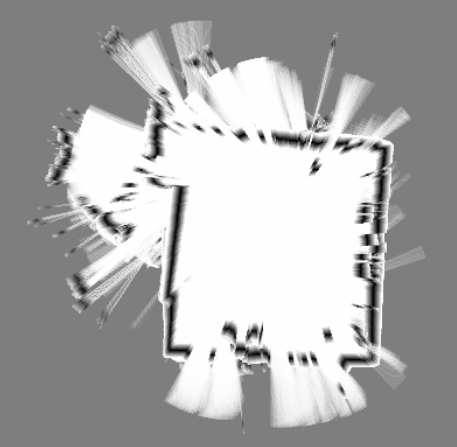
\includegraphics[width=0.45\linewidth, height=7cm]{SLAM/noodo1ROOM}}	
	\hspace{0.01\linewidth}
	\subfigure[Map van 1 kamer, gegenereerd met odometrie]{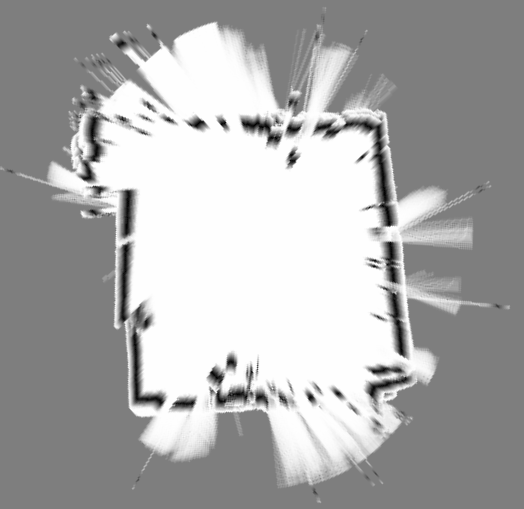
\includegraphics[width=0.45\linewidth, height=7cm]{SLAM/odo1ROOM}}
	
	\subfigure[Map van 3 kamers, gegenereerd zonder odometrie]{\includegraphics[width=0.45\linewidth, height=6cm]{SLAM/noodo3ROOMS}}
	\hspace{0.01\linewidth}
	\subfigure[Map van 3 kamers, gegenereerd met odometrie]{\includegraphics[width=0.45\linewidth, height=6cm]{SLAM/odo3ROOMS}}
	\caption{Vergelijking tussen de prestatie van BreezySLAM met en zonder odometrie. Om deze mappen te genereren werd het meermaals bezoeken van eenzelfde plaats vermeden. De prestatie van BreezySLAM met en zonder odometrie is ongeveer dezelfde wanneer een kleine ruimte gemapt wordt. Als drie aaneensluitende ruimtes gemapt moeten worden roteren ze wat ten opzichte van elkaar wanneer geen odometrie wordt gebruikt. Als wel odometrie wordt gebruikt, liggen de kamers correcter ten opzichte van elkaar.}\label{fig:BreezyRes}
\end{figure}

\begin{figure}
	\centering
	\subfigure[Loop-closing zonder odometrie]{\includegraphics[width=0.45\linewidth, height=7cm]{SLAM/loopclosure}}	
	\hspace{0.01\linewidth}
	\subfigure[Loop-closing met odometrie]{\includegraphics[width=0.45\linewidth, height=7cm]{SLAM/odoloopclosing}}
	\caption{Loop-closing vergeleken voor BreezySLAM zonder(a) en met(b) odometrie. Het meermaals bezoeken van eenzelfde plaats blijft een probleem, ook wanneer odometrie gebruikt wordt.} \label{fig:loopclosing2}
\end{figure}


% !TeX spellcheck = nl_NL
\chapter{Conclusie}
Deze thesis heeft als einddoel het realiseren van een autonome quadcopter die in staat is om zijn omgeving in kaart te brengen. Het einddoel is dus in twee delen op te splitsen. In het eerste deel moet de stabiliteit van het autonome platform verbeterd worden door de sturing van de quadcopter te optimaliseren. De conclusies van dit deel worden verder besproken in sectie \ref{sec:concOpt}. In het tweede deel moet een gepast SLAM algoritme gezocht worden en moet het platform worden uitgebreid om omgevingsmapping mogelijk te maken. De conclusie met betrekking tot dit deel worden verder besproken in \ref{sec:concSLAM}. Om dit hoofdstuk af te sluiten worden enkele suggesties opgesomd voor toekomstige werken.

\section{Optimalisatie} \label{sec:concOpt}
Er zijn verschillende stappen ondernomen om het vlieggedrag van het platform stabieler te maken. Deze stappen worden hieronder overlopen.

\npar Het platform gebruikt optical flow om drift te detecteren en vervolgens te compenseren. Uit de evaluatie van het platform is gebleken dat de huidige hardware over onvoldoende rekenkracht beschikt om met hoge snelheid en hoge nauwkeurigheid drift te detecteren. De zware berekeningen die hiervoor nodig zijn, zijn om die reden verlegd naar de PC. De features waaruit de optical flow vectoren worden berekend, worden oorspronkelijk geselecteerd met de FAST detector. Omdat rekenkracht niet langer een probleem vormt, is de GFTT detector uitgeprobeerd, een andere, preciezere detector die meer rekenkracht eist. Na vergelijking met de FAST detector is gebleken dat GFTT duidelijk beter presteert, vooral wanneer de beelden, waarover optical flow berekend wordt, wazig zijn. Ik concludeer dat drift nu een stuk nauwkeuriger wordt gedetecteerd. Hierdoor kan drift dan ook beter gecompenseerd worden.

\npar Wanneer gebruik wordt gemaakt van een PID-regelaar moet het correctiesignaal op de juiste manier teruggevoerd worden. De hoogte wordt geregeld door de aangelegde throttle. Er is verondersteld dat er een ideale waarde voor deze throttle bestaat die ervoor zorgt dat het platform op \'e\'en hoogte blijft vliegen. Deze waarde is nodig om het correctiesignaal van de PID-regelaar bij op te tellen. De ideale throttlewaarde hangt echter af van de resterende batterijspanning. Hoe lager de spanning, hoe hoger deze waarde zal zijn. Als oplossing wordt tijdens het opstijgen een schatting gemaakt van deze ideale throttlewaarde. Dit door de versnelling van het platform in z-richting te meten. Om op een vaste hoogte te kunnen vliegen moet de fout op de schatting nog gecompenseerd worden door de integrerende term van de PID-regelaar. Ik besluit dat voor een goeie hoogteregeling vanaf het begin van de vlucht een goede schatting van de ideale throttlewaarde essentieel is. Door optimale PID-parameters te gebruiken, is de hoogteregeling in het vervolg van de vlucht ook beter.

\npar Er is aangetoond dat een goede hoogteregeling essentieel is indien voor driftdetectie optical flow wordt gebruikt. Wanneer het platform stijgt of daalt, kan met optical flow drift gedetecteerd worden die er eigenlijk niet is. Om dit probleem aan te pakken, wordt gebruik gemaakt van een functiegenerator die de gewenste hoogte gestaag naar de eigenlijke setpoint laat convergeren. Omdat de hoogteveranderingen nu allemaal trager verlopen, is de valse drift die optical flow detecteert een stuk kleiner. De compensatie die het platform uitvoert om deze valse drift tegen te gaan is dan ook kleiner. Hierdoor is het platform dan weer wat stabieler. Bovendien zorgt het gebruik van de functiegenerator er ook voor dat de hoogte van het platform minder overshoot heeft. Dit is te verklaren door het feit dat de functiegenerator het platform een maximale snelheid oplegt waarmee het mag stijgen of dalen. Ik concludeer dat het gebruik van de functiegenerator zowel op vlak van hoogte als op vlak van positie bijdraagt aan een stabieler vlieggedrag.

\npar De positieregelaar is aangepast en vervolgens ook geoptimaliseerd. Er wordt gekozen voor een PI-regelaar die de snelheid van het platform regelt. Wanneer het platform op eenzelfde plaats moet blijven vliegen, wordt de gewenste snelheid op nul gehouden. Wanneer een nieuwe positie bereikt moet worden kan de snelheid in de richting van deze nieuwe positie aangepast worden. Ik besluit dat dit een goeie aanpak is om de positie van het platform te regelen.

\npar Mijn conclusie is dat de combinatie van bovenstaande optimalisaties het platform voldoende stabiel maakt om over te gaan naar het tweede deel van deze thesis, het in kaart brengen van de omgeving van het platform.

\section{Omgevingsmapping} \label{sec:concSLAM}
\npar Het tweede deel van deze thesis gaat over omgevingsmapping met SLAM. Er is op zoek gegaan naar een geschikt SLAM algoritme om aan omgevingsmapping te doen. Hiervoor zijn twee paradigma's met elkaar vergeleken. SLAM algoritmes met Extended Kalman filters en algoritmes met Particle filters. Omwille van de beperkte rekenkracht op het platform, is voor het laatste van de twee gekozen. Binnen dit paradigma zijn nog steeds heel veel verschillende implementaties mogelijk. Als eerste is {HectorSLAM} geprobeerd, dit algoritme houdt rekening met alle zes vrijheidsgraden van het platform. {HectorSLAM} vereist het gebruik van een ROS raamwerk. Omdat het niet is gelukt om dit werkende te krijgen, is er verder gezocht naar een andere implementatie. Vervolgens is er geprobeerd om {TinySLAM} te implementeren. Dit is een vrij licht SLAM algoritme dat uit een heel beperkt aantal lijnen code bestaat. Het is echter niet gelukt om {TinySLAM} te implementeren omdat de interface van dit algoritme nogal cryptisch geschreven is. Uiteindelijk is er voor {BreezySLAM} gekozen. Dit algoritme is gebaseerd op {TinySLAM}, maar heeft wel een goeie interface.

\npar Om te beginnen is {BreezySLAM} in de architectuur van het platform ge\"integreerd. {BreezySLAM} kan zowel met als zonder odometrie gebruikt worden. De prestaties van deze twee mogelijkheden zijn dan ook met elkaar vergeleken. Uit dit onderzoek blijkt dat {BreezySLAM} goed presteert zolang de te verkennen ruimte klein blijft en eenzelfde plaats niet meer dan eens wordt bezocht. In de praktijk is bij het verkennen van een ruimte het opnieuw bezoeken van eenzelfde plaats vaak onvermijdelijk. Ik kan concluderen dat het gekozen SLAM algoritme niet ideaal is om onbekende ruimtes te verkennen. Desondanks is er wel bewezen dat omgevingsmapping met het platform mogelijk is.

\npar Mijn conclusie is dat omgevingsmapping met een low-cost quadcopter zeker kan. Met goedkope hardware kunnen voldoende nauwkeurige mappen gemaakt worden van kleine gebouwen. Voor grotere gebouwen, eist SLAM echter wel heel veel geheugen. Het is dan ook beter om op de quadcopter enkel een lokale map bij te houden, terwijl een globale map extern wordt gemaakt. De lokale map kan gebruikt worden door de quadcopter voor het ontwijken van obstakels, de globale map kan dan gebruikt voor routeplanning op een hoger niveau. 

\npar Quadcopters zullen in de toekomst ongetwijfeld ingezet worden voor search and rescue missies. In tegenstelling tot grondrobots die niet geschikt zijn voor ruw terrein, kunnen quadcopters overal vliegen. Bij reddingsoperaties kan een nauwkeurige 3D map van een volledig gebouw van onschatbare waarde zijn. Hoe sneller deze map er is, hoe beter. Het lijkt dan ook logisch dat in de toekomst meerdere quadcopters zullen samenwerken om een gebouw nog sneller in kaart te brengen.

\section{Toekomstig werk}
Het platform is aan een update toe. Een aantal crashes hebben het nogal beschadigd. Het frame is wat geplooid, het centrum voor de elektronica moest hier en daar samen gelijmd worden. Er wordt aangeraden om een nieuw frame te ontwerpen, met een meer robuuste kern. De lijst van hardwarecomponenten die erop moeten is gekend. Het is dus enkel nog een kwestie om overal genoeg plaats te voorzien en ervoor te zorgen dat alles met vijzen bevestigd kan worden. Als het frame volledig recht zou zijn, dan zal het toestel in staat zijn mooi verticaal op te stijgen, in deze thesis is dit niet het geval en is dit ook de oorzaak geweest van meerdere crashes.

\npar De gebruikte autopilot, de APM 1.4 is verouderd. Tegenwoordig is de APM 2.6 reeds beschikbaar. Deze autopilot zorgt sowieso al voor een stuk stabieler vlieggedrag omdat er minder drift op zijn sensoren zit. Bovendien kan er ook een optical flow chip aan verbonden worden, waardoor de RPi veel meer rekenkracht overhoudt voor het verkennen en mappen van de omgeving.

\npar Op vlak van software wordt er aangeraden over te schakelen naar het ROS raamwerk. {HectorSLAM} kan dan gebruikt worden voor omgevingsmapping. Dit algoritme houdt rekening met alle zes vrijheidsgraden van het platform. Als het CPU-gebruik dit toelaat kan zelfs nog overgestapt worden naar een 3D SLAM algoritme zoals {OctoSLAM} \cite{paper:OctoSLAM}. Als dit niet blijkt te lukken, kan de laserscanner ook aan een lagere frequentie gebruikt worden dan zijn maximumfrequentie \SI{10}{\Hz}.

% De bibliografie
% Het bibliografisch opmaak bestand.
\bibliographystyle{IEEEtran}
%\bibpunct{[}{]}{,}{n}{,}{,}
\bibliography{bibliodatabase}


\backmatter


\appendix
% lege pagina (!!)
\pagestyle{empty}
\newpage
\vfil\null
\newpage

%kaft
\newpage
\vfil\null
\newpage

\end{document}


